\documentclass{book}
\usepackage[a4paper,top=2.5cm,bottom=2.5cm,left=2.5cm,right=2.5cm]{geometry}
\usepackage{makeidx}
\usepackage{natbib}
\usepackage{graphicx}
\usepackage{multicol}
\usepackage{float}
\usepackage{listings}
\usepackage{color}
\usepackage{ifthen}
\usepackage[table]{xcolor}
\usepackage{textcomp}
\usepackage{alltt}
\usepackage{ifpdf}
\ifpdf
\usepackage[pdftex,
            pagebackref=true,
            colorlinks=true,
            linkcolor=blue,
            unicode
           ]{hyperref}
\else
\usepackage[ps2pdf,
            pagebackref=true,
            colorlinks=true,
            linkcolor=blue,
            unicode
           ]{hyperref}
\usepackage{pspicture}
\fi
\usepackage[utf8]{inputenc}
\usepackage{mathptmx}
\usepackage[scaled=.90]{helvet}
\usepackage{courier}
\usepackage{sectsty}
\usepackage{amssymb}
\usepackage[titles]{tocloft}
\usepackage{doxygen}
\lstset{language=C++,inputencoding=utf8,basicstyle=\footnotesize,breaklines=true,breakatwhitespace=true,tabsize=2,numbers=left }
\makeindex
\setcounter{tocdepth}{3}
\renewcommand{\footrulewidth}{0.4pt}
\renewcommand{\familydefault}{\sfdefault}
\hfuzz=15pt
\setlength{\emergencystretch}{15pt}
\hbadness=750
\tolerance=750
\begin{document}
\hypersetup{pageanchor=false,citecolor=blue}
\begin{titlepage}
\vspace*{7cm}
\begin{center}
{\Large R\-G\-B\-D360 }\\
\vspace*{1cm}
{\large Generated by Doxygen 1.8.3.1}\\
\vspace*{0.5cm}
{\small Wed Dec 18 2013 13:08:19}\\
\end{center}
\end{titlepage}
\clearemptydoublepage
\pagenumbering{roman}
\tableofcontents
\clearemptydoublepage
\pagenumbering{arabic}
\hypersetup{pageanchor=true,citecolor=blue}
\chapter{Documentation Overview}
\label{index}\hypertarget{index}{}\hypertarget{index_intro_sec}{}\section{Introduction}\label{index_intro_sec}
This project contains the basic functionality to acquire images from a R\-G\-B-\/\-D sensor using Open\-N\-I2, and to perform some basic operations. Functions to serialize (load/save) such images, to undistort the depth images, or building point clouds are also provided. Two applications are provided.\hypertarget{index_project_sec}{}\section{Project tree}\label{index_project_sec}
The main functionality of this project is implemented in a set of header files that are found in the directories\-: \par
 'frame\-R\-G\-B\-D/'
\begin{DoxyItemize}
\item Frame\-R\-G\-B\-D.\-h
\item Cloud\-R\-G\-B\-D.\-h
\item Cloud\-Visualization.\-h and 'grabber/'
\item \hyperlink{RGBDGrabber_8h_source}{R\-G\-B\-D\-Grabber.\-h} The project applications are found in the directory 'apps/'
\item Calibration/ \par
 -\/$>$ Contains the applications to calibrate the extrinsic parameters of the sensor
\item Grabber/ \par
 -\/$>$ Grab and serialize the omnidirectional R\-G\-B-\/\-D image
\end{DoxyItemize}\hypertarget{index_dependencies_sec}{}\section{Dependencies}\label{index_dependencies_sec}
This project integrates several open-\/source libraries to build the whole solution. The main dependencies are\-:
\begin{DoxyItemize}
\item Open\-C\-V\-: \href{http://opencv.org/}{\tt http\-://opencv.\-org/}
\item P\-C\-L\-: \href{http://pointclouds.org/}{\tt http\-://pointclouds.\-org/}
\item Open\-N\-I2\-: \href{http://www.openni.org/}{\tt http\-://www.\-openni.\-org/} (This library is needed to open and read the sensor)
\end{DoxyItemize}\hypertarget{index_install_sec}{}\section{Installation}\label{index_install_sec}
This project has been implemented and tested in Ubuntu 12.\-04 and 13.\-04. This project contains a C\-Malelists.\-txt file to facilitate the integration of the different dependencies. Thus, the program C\-Make is required to produce the Makefile configuration file for compilation. To compile the source code the above dependencies must be installed first. After that, the following steps will guide you to compile the project. \begin{DoxyVerb}cd yourPathTo/RGBD360
\end{DoxyVerb}
 \begin{DoxyVerb}  - Generate the Makefile with CMake.
       -# Open CMake (the following instructions are for cmake-gui).
       -# Set the source directory to RGBD360 and the build directory to RGBD360/build.
       -# Set OpenCV_DIR, PCL_DIR and MRPT_DIR to the OpenCV, PCL and MRPT build directories respectively.
       -# Set the application packages to build (Grabber, Visualizer, etc.). To reckon which packages you need, go to the next section to find out a more detailed description of each package's applications.
       -# Configure.
       -# Generate.

  - Compile the RGBD360 project.
       -# Go to the directory RGBD360/build/
       -# Compile with 'make'.
\end{DoxyVerb}
\hypertarget{index_usage_sec}{}\section{Software usage}\label{index_usage_sec}
After compiling the project, a number of directories containing the different application packages will be created. The applications of these packages are described below (a brief description of each application and its syntaxis is shown on executing ./application -\/h')\-: \hypertarget{index_Calibration}{}\subsection{Calibration}\label{index_Calibration}
This package contains the applications to calibrate the extrinsic parameters of the sensor

\begin{DoxyAuthor}{Author}
Eduardo Fernandez-\/\-Moral 
\end{DoxyAuthor}

\chapter{Hierarchical Index}
\section{Class Hierarchy}
This inheritance list is sorted roughly, but not completely, alphabetically\-:\begin{DoxyCompactList}
\item \contentsline{section}{Calib360}{\pageref{classCalib360}}{}
\begin{DoxyCompactList}
\item \contentsline{section}{Calibrator}{\pageref{classCalibrator}}{}
\end{DoxyCompactList}
\item \contentsline{section}{Cloud\-Grabber}{\pageref{classCloudGrabber}}{}
\item \contentsline{section}{Filter\-Point\-Cloud}{\pageref{classFilterPointCloud}}{}
\item \contentsline{section}{Frame360}{\pageref{classFrame360}}{}
\item \contentsline{section}{Frame360\-\_\-\-Visualizer}{\pageref{classFrame360__Visualizer}}{}
\item \contentsline{section}{Graph\-Optimizer}{\pageref{classGraphOptimizer}}{}
\item \contentsline{section}{Loop\-Closure360}{\pageref{classLoopClosure360}}{}
\item \contentsline{section}{Map360}{\pageref{structMap360}}{}
\item \contentsline{section}{Map360\-\_\-\-Visualizer}{\pageref{classMap360__Visualizer}}{}
\item \contentsline{section}{Register\-R\-G\-B\-D360}{\pageref{classRegisterRGBD360}}{}
\item \contentsline{section}{Relocalizer360}{\pageref{classRelocalizer360}}{}
\item \contentsline{section}{Topological\-Map360}{\pageref{classTopologicalMap360}}{}
\item \contentsline{section}{Visualizer\-R\-G\-B\-D360}{\pageref{classVisualizerRGBD360}}{}
\end{DoxyCompactList}

\chapter{Class Index}
\section{Class List}
Here are the classes, structs, unions and interfaces with brief descriptions\-:\begin{DoxyCompactList}
\item\contentsline{section}{\hyperlink{classRGBDGrabber}{R\-G\-B\-D\-Grabber} }{\pageref{classRGBDGrabber}}{}
\item\contentsline{section}{\hyperlink{classRGBDGrabber__OpenNI2}{R\-G\-B\-D\-Grabber\-\_\-\-Open\-N\-I2} }{\pageref{classRGBDGrabber__OpenNI2}}{}
\end{DoxyCompactList}

\chapter{Class Documentation}
\hypertarget{classCalib360}{\section{Calib360 Class Reference}
\label{classCalib360}\index{Calib360@{Calib360}}
}


{\ttfamily \#include $<$Calib360.\-h$>$}

Inheritance diagram for Calib360\-:\begin{figure}[H]
\begin{center}
\leavevmode
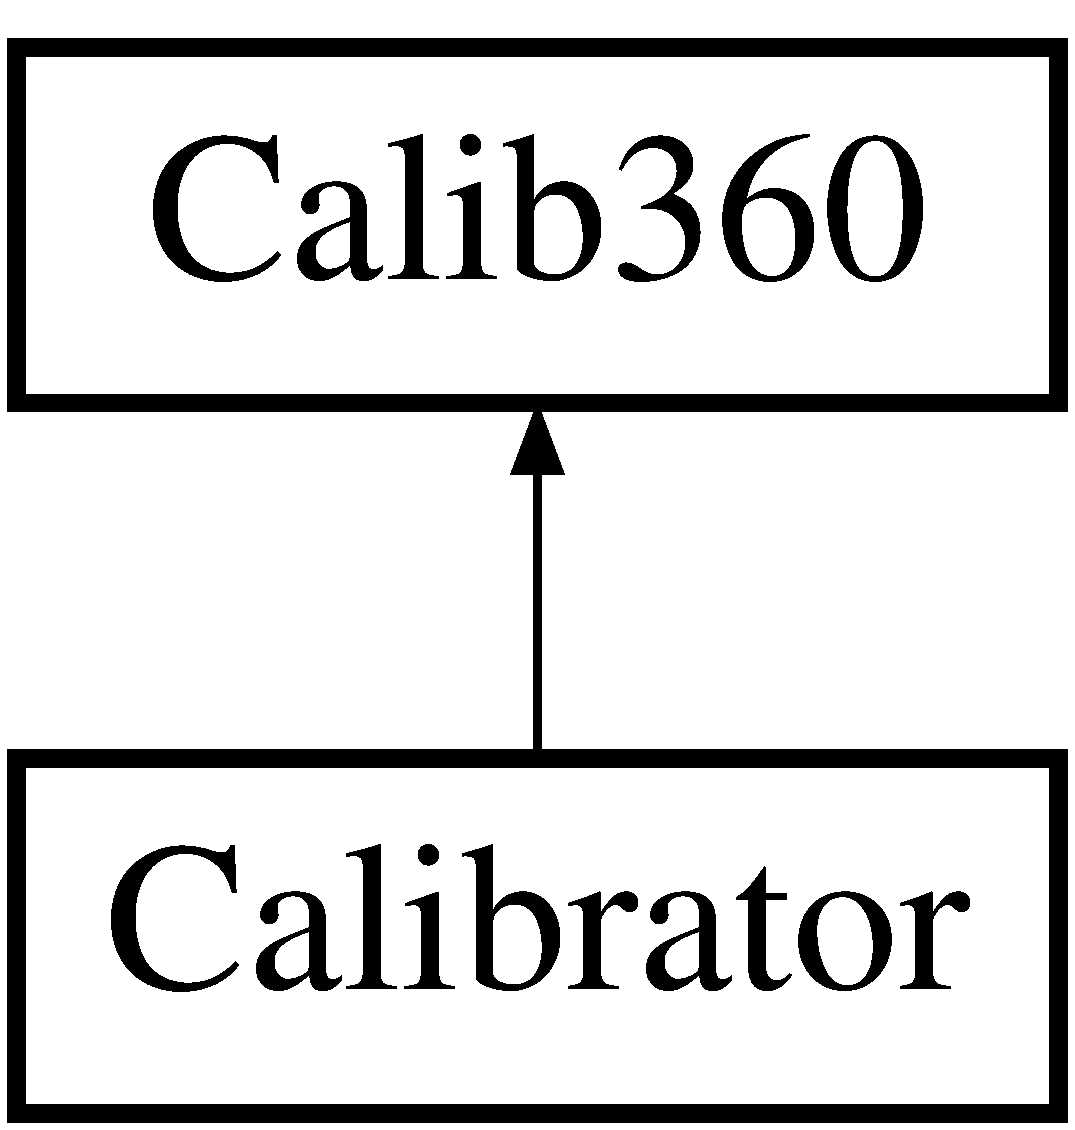
\includegraphics[height=2.000000cm]{classCalib360}
\end{center}
\end{figure}
\subsection*{Public Types}
\begin{DoxyCompactItemize}
\item 
enum \hyperlink{classCalib360_a323701c4815353e02f79ce58a9ef2e12}{Resolution} \{ {\bfseries V\-G\-A} = 1, 
{\bfseries Q\-V\-G\-A} = 2, 
{\bfseries Q\-Q\-V\-G\-A} = 4
 \}
\end{DoxyCompactItemize}
\subsection*{Public Member Functions}
\begin{DoxyCompactItemize}
\item 
\hyperlink{classCalib360_ab2365a4a8b4453258ff2664aa9d80a11}{Calib360} (\hyperlink{classCalib360_a323701c4815353e02f79ce58a9ef2e12}{Resolution} res=Q\-V\-G\-A)
\item 
Eigen\-::\-Matrix4f \hyperlink{classCalib360_a700a92c794bceaacbb200eacd281fda1}{get\-Rt\-\_\-id} (int id) const 
\item 
void \hyperlink{classCalib360_a8f9c38de4304edacc433a1e3b6e54e41}{set\-Rt\-\_\-id} (int id, Eigen\-::\-Matrix4f \&Rt)
\item 
void \hyperlink{classCalib360_a01c3fc478c6614f2a78db01575223940}{load\-Intrinsic\-Calibration} (std\-::string path\-To\-Intrinsic\-Model=\char`\"{}\char`\"{})
\item 
void \hyperlink{classCalib360_ad9833ea56bb48ff7a488ce8d77566ca6}{load\-Extrinsic\-Calibration} (std\-::string path\-To\-Extrinsic\-Model=\char`\"{}\char`\"{})
\end{DoxyCompactItemize}
\subsection*{Public Attributes}
\begin{DoxyCompactItemize}
\item 
std\-::vector\\*
$<$ clams\-::\-Discrete\-Depth\-Distortion\-Model $>$ \hyperlink{classCalib360_aa2e0b8086073711793812d4253b272ec}{intrinsic\-\_\-model\-\_\-}
\item 
Eigen\-::\-Matrix4f \hyperlink{classCalib360_a61dacdf729067dcea6d270f79e628b83}{Rt\-\_\-} \mbox{[}N\-U\-M\-\_\-\-A\-S\-U\-S\-\_\-\-S\-E\-N\-S\-O\-R\-S\mbox{]}
\item 
Eigen\-::\-Matrix4f \hyperlink{classCalib360_a179de6c9f42a6b1bbd4cfda04e857bda}{Rt\-\_\-inv} \mbox{[}N\-U\-M\-\_\-\-A\-S\-U\-S\-\_\-\-S\-E\-N\-S\-O\-R\-S\mbox{]}
\item 
Eigen\-::\-Matrix3f \hyperlink{classCalib360_a27be5251d6ba2a81b6be00424c82b736}{camera\-Matrix}
\item 
\hypertarget{classCalib360_ac6491eb444561b47451f09d6bac3b071}{enum \hyperlink{classCalib360_a323701c4815353e02f79ce58a9ef2e12}{Calib360\-::\-Resolution} {\bfseries resolution}}\label{classCalib360_ac6491eb444561b47451f09d6bac3b071}

\end{DoxyCompactItemize}


\subsection{Detailed Description}
This class contains the functionality to load the calibration parameters of the omnidirectional R\-G\-B-\/\-D device (R\-G\-B\-D360). The intrinsic calibration is loaded from previous models obtained with C\-L\-A\-M\-S (\href{http://cs.stanford.edu/people/teichman/octo/clams/}{\tt http\-://cs.\-stanford.\-edu/people/teichman/octo/clams/}). The extrinsic calibration is loaded from the models obtained with the Calibration programs. 

\subsection{Member Enumeration Documentation}
\hypertarget{classCalib360_a323701c4815353e02f79ce58a9ef2e12}{\index{Calib360@{Calib360}!Resolution@{Resolution}}
\index{Resolution@{Resolution}!Calib360@{Calib360}}
\subsubsection[{Resolution}]{\setlength{\rightskip}{0pt plus 5cm}enum {\bf Calib360\-::\-Resolution}}}\label{classCalib360_a323701c4815353e02f79ce58a9ef2e12}
Resolution mode of the device (default is Q\-V\-G\-A = 320x240) 

\subsection{Constructor \& Destructor Documentation}
\hypertarget{classCalib360_ab2365a4a8b4453258ff2664aa9d80a11}{\index{Calib360@{Calib360}!Calib360@{Calib360}}
\index{Calib360@{Calib360}!Calib360@{Calib360}}
\subsubsection[{Calib360}]{\setlength{\rightskip}{0pt plus 5cm}Calib360\-::\-Calib360 (
\begin{DoxyParamCaption}
\item[{{\bf Resolution}}]{res = {\ttfamily QVGA}}
\end{DoxyParamCaption}
)\hspace{0.3cm}{\ttfamily [inline]}}}\label{classCalib360_ab2365a4a8b4453258ff2664aa9d80a11}
Constructor 

\subsection{Member Function Documentation}
\hypertarget{classCalib360_a700a92c794bceaacbb200eacd281fda1}{\index{Calib360@{Calib360}!get\-Rt\-\_\-id@{get\-Rt\-\_\-id}}
\index{get\-Rt\-\_\-id@{get\-Rt\-\_\-id}!Calib360@{Calib360}}
\subsubsection[{get\-Rt\-\_\-id}]{\setlength{\rightskip}{0pt plus 5cm}Eigen\-::\-Matrix4f Calib360\-::get\-Rt\-\_\-id (
\begin{DoxyParamCaption}
\item[{int}]{id}
\end{DoxyParamCaption}
) const\hspace{0.3cm}{\ttfamily [inline]}}}\label{classCalib360_a700a92c794bceaacbb200eacd281fda1}
Return the relative position of the camera 'id' \hypertarget{classCalib360_ad9833ea56bb48ff7a488ce8d77566ca6}{\index{Calib360@{Calib360}!load\-Extrinsic\-Calibration@{load\-Extrinsic\-Calibration}}
\index{load\-Extrinsic\-Calibration@{load\-Extrinsic\-Calibration}!Calib360@{Calib360}}
\subsubsection[{load\-Extrinsic\-Calibration}]{\setlength{\rightskip}{0pt plus 5cm}void Calib360\-::load\-Extrinsic\-Calibration (
\begin{DoxyParamCaption}
\item[{std\-::string}]{path\-To\-Extrinsic\-Model = {\ttfamily \char`\"{}\char`\"{}}}
\end{DoxyParamCaption}
)\hspace{0.3cm}{\ttfamily [inline]}}}\label{classCalib360_ad9833ea56bb48ff7a488ce8d77566ca6}
Load the extrinsic calibration matrices (relative poses) corresponding to each Asus X\-P\-L \hypertarget{classCalib360_a01c3fc478c6614f2a78db01575223940}{\index{Calib360@{Calib360}!load\-Intrinsic\-Calibration@{load\-Intrinsic\-Calibration}}
\index{load\-Intrinsic\-Calibration@{load\-Intrinsic\-Calibration}!Calib360@{Calib360}}
\subsubsection[{load\-Intrinsic\-Calibration}]{\setlength{\rightskip}{0pt plus 5cm}void Calib360\-::load\-Intrinsic\-Calibration (
\begin{DoxyParamCaption}
\item[{std\-::string}]{path\-To\-Intrinsic\-Model = {\ttfamily \char`\"{}\char`\"{}}}
\end{DoxyParamCaption}
)\hspace{0.3cm}{\ttfamily [inline]}}}\label{classCalib360_a01c3fc478c6614f2a78db01575223940}
Load the intrinsic calibration models corresponding to each Asus X\-P\-L \hypertarget{classCalib360_a8f9c38de4304edacc433a1e3b6e54e41}{\index{Calib360@{Calib360}!set\-Rt\-\_\-id@{set\-Rt\-\_\-id}}
\index{set\-Rt\-\_\-id@{set\-Rt\-\_\-id}!Calib360@{Calib360}}
\subsubsection[{set\-Rt\-\_\-id}]{\setlength{\rightskip}{0pt plus 5cm}void Calib360\-::set\-Rt\-\_\-id (
\begin{DoxyParamCaption}
\item[{int}]{id, }
\item[{Eigen\-::\-Matrix4f \&}]{Rt}
\end{DoxyParamCaption}
)\hspace{0.3cm}{\ttfamily [inline]}}}\label{classCalib360_a8f9c38de4304edacc433a1e3b6e54e41}
Stitch both the R\-G\-B and the depth images corresponding to the sensor 'sensor\-\_\-id' 

\subsection{Member Data Documentation}
\hypertarget{classCalib360_a27be5251d6ba2a81b6be00424c82b736}{\index{Calib360@{Calib360}!camera\-Matrix@{camera\-Matrix}}
\index{camera\-Matrix@{camera\-Matrix}!Calib360@{Calib360}}
\subsubsection[{camera\-Matrix}]{\setlength{\rightskip}{0pt plus 5cm}Eigen\-::\-Matrix3f Calib360\-::camera\-Matrix}}\label{classCalib360_a27be5251d6ba2a81b6be00424c82b736}
The intrinsic pinhole camera model. W\-A\-R\-N\-I\-N\-G\-: this is set fdepending on the chosen resolution (we use 320x240) \hypertarget{classCalib360_aa2e0b8086073711793812d4253b272ec}{\index{Calib360@{Calib360}!intrinsic\-\_\-model\-\_\-@{intrinsic\-\_\-model\-\_\-}}
\index{intrinsic\-\_\-model\-\_\-@{intrinsic\-\_\-model\-\_\-}!Calib360@{Calib360}}
\subsubsection[{intrinsic\-\_\-model\-\_\-}]{\setlength{\rightskip}{0pt plus 5cm}std\-::vector$<$clams\-::\-Discrete\-Depth\-Distortion\-Model$>$ Calib360\-::intrinsic\-\_\-model\-\_\-}}\label{classCalib360_aa2e0b8086073711793812d4253b272ec}
The intrinsic depth distortion models corresponding to each Asus X\-P\-L \hypertarget{classCalib360_a61dacdf729067dcea6d270f79e628b83}{\index{Calib360@{Calib360}!Rt\-\_\-@{Rt\-\_\-}}
\index{Rt\-\_\-@{Rt\-\_\-}!Calib360@{Calib360}}
\subsubsection[{Rt\-\_\-}]{\setlength{\rightskip}{0pt plus 5cm}Eigen\-::\-Matrix4f Calib360\-::\-Rt\-\_\-\mbox{[}N\-U\-M\-\_\-\-A\-S\-U\-S\-\_\-\-S\-E\-N\-S\-O\-R\-S\mbox{]}}}\label{classCalib360_a61dacdf729067dcea6d270f79e628b83}
The extrinsic parameters (relative position) of to each Asus X\-P\-L \hypertarget{classCalib360_a179de6c9f42a6b1bbd4cfda04e857bda}{\index{Calib360@{Calib360}!Rt\-\_\-inv@{Rt\-\_\-inv}}
\index{Rt\-\_\-inv@{Rt\-\_\-inv}!Calib360@{Calib360}}
\subsubsection[{Rt\-\_\-inv}]{\setlength{\rightskip}{0pt plus 5cm}Eigen\-::\-Matrix4f Calib360\-::\-Rt\-\_\-inv\mbox{[}N\-U\-M\-\_\-\-A\-S\-U\-S\-\_\-\-S\-E\-N\-S\-O\-R\-S\mbox{]}}}\label{classCalib360_a179de6c9f42a6b1bbd4cfda04e857bda}
The inverse matrices of each Asus X\-P\-L's relative position 

The documentation for this class was generated from the following file\-:\begin{DoxyCompactItemize}
\item 
include/Calib360.\-h\end{DoxyCompactItemize}

\hypertarget{classCalibrator}{\section{Calibrator Class Reference}
\label{classCalibrator}\index{Calibrator@{Calibrator}}
}


{\ttfamily \#include $<$Calibrator.\-h$>$}

Inheritance diagram for Calibrator\-:\begin{figure}[H]
\begin{center}
\leavevmode
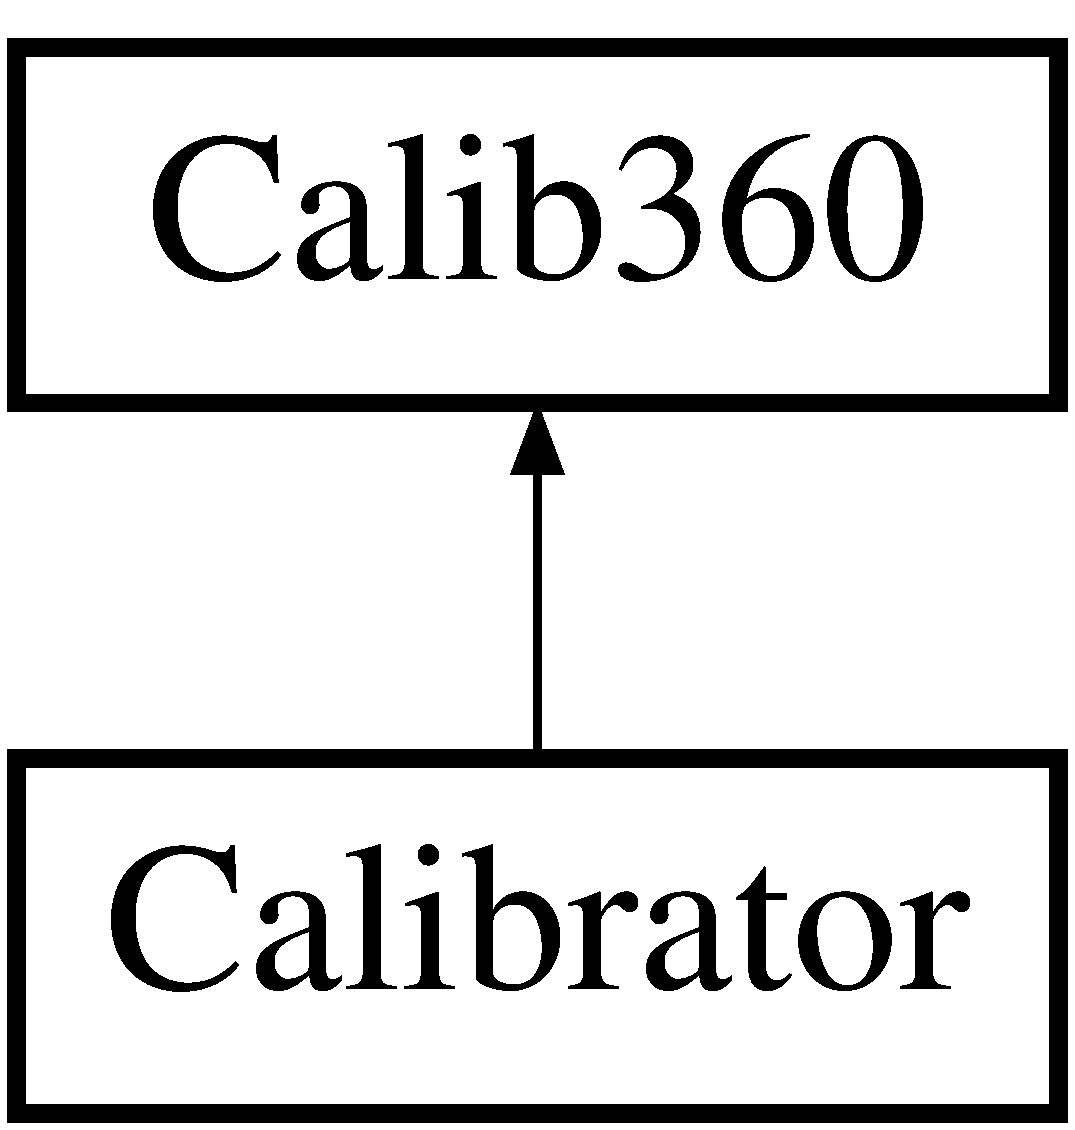
\includegraphics[height=2.000000cm]{classCalibrator}
\end{center}
\end{figure}
\subsection*{Public Member Functions}
\begin{DoxyCompactItemize}
\item 
void \hyperlink{classCalibrator_a749ed4be8cd2b66416b954af8ef24a9f}{load\-Construction\-Specs} ()
\item 
void \hyperlink{classCalibrator_a8f5f7422d896db20aad3812051eeb92e}{save\-Plane\-Correspondences} (std\-::string \&plane\-Corresp\-Directory)
\item 
void \hyperlink{classCalibrator_a14899494a37a1e838e2f6717a7114a8f}{load\-Plane\-Correspondences} (const std\-::string plane\-Corresp\-Directory)
\item 
float \hyperlink{classCalibrator_ac95df4664b1ca9b1188caf9a877348d5}{calc\-Corresp\-Rot\-Error} (Eigen\-::\-Matrix4f $\ast$\hyperlink{classCalib360_a61dacdf729067dcea6d270f79e628b83}{Rt\-\_\-})
\item 
float \hyperlink{classCalibrator_ae6aef26dc04a71762fac9d4dab2513c5}{calc\-Corresp\-Trans\-Error} (Eigen\-::\-Matrix4f $\ast$\hyperlink{classCalib360_a61dacdf729067dcea6d270f79e628b83}{Rt\-\_\-})
\item 
void \hyperlink{classCalibrator_a958435e23a9f93cfac798925b1653171}{Calibrate\-Rotation} ()
\item 
void \hyperlink{classCalibrator_af896bad41d28ff7ce20d77361414edc6}{Calibrate\-Translation} ()
\item 
void \hyperlink{classCalibrator_a337977f493659555f73fb476c686bb3c}{Calibrate} ()
\end{DoxyCompactItemize}
\subsection*{Public Attributes}
\begin{DoxyCompactItemize}
\item 
Eigen\-::\-Matrix4f \hyperlink{classCalibrator_ada5174649775a64c103833f87d90ec3e}{Rt\-\_\-specs} \mbox{[}N\-U\-M\-\_\-\-A\-S\-U\-S\-\_\-\-S\-E\-N\-S\-O\-R\-S\mbox{]}
\item 
Eigen\-::\-Matrix4f \hyperlink{classCalibrator_a664327b52485de0d402bbc896ce1233f}{Rt\-\_\-estimated} \mbox{[}N\-U\-M\-\_\-\-A\-S\-U\-S\-\_\-\-S\-E\-N\-S\-O\-R\-S\mbox{]}
\end{DoxyCompactItemize}
\subsection*{Private Attributes}
\begin{DoxyCompactItemize}
\item 
std\-::map$<$ unsigned, std\-::map\\*
$<$ unsigned, \\*
mrpt\-::math\-::\-C\-Matrix\-Double $>$ $>$ \hyperlink{classCalibrator_aa11e0d4221b509241235755dde78e3cc}{mm\-Correspondences}
\end{DoxyCompactItemize}
\subsection*{Additional Inherited Members}


\subsection{Detailed Description}
This class contains the functionality to calibrate the extrinsic parameters of the omnidirectional R\-G\-B-\/\-D device (R\-G\-B\-D360). This extrinsic calibration is obtained by matching planes that are observed by several Asus X\-P\-L sensors at the same time. 

\subsection{Member Function Documentation}
\hypertarget{classCalibrator_ac95df4664b1ca9b1188caf9a877348d5}{\index{Calibrator@{Calibrator}!calc\-Corresp\-Rot\-Error@{calc\-Corresp\-Rot\-Error}}
\index{calc\-Corresp\-Rot\-Error@{calc\-Corresp\-Rot\-Error}!Calibrator@{Calibrator}}
\subsubsection[{calc\-Corresp\-Rot\-Error}]{\setlength{\rightskip}{0pt plus 5cm}float Calibrator\-::calc\-Corresp\-Rot\-Error (
\begin{DoxyParamCaption}
\item[{Eigen\-::\-Matrix4f $\ast$}]{Rt\-\_\-}
\end{DoxyParamCaption}
)\hspace{0.3cm}{\ttfamily [inline]}}}\label{classCalibrator_ac95df4664b1ca9b1188caf9a877348d5}
Get the sum of squared rotational errors for the input extrinsic matrices. T\-O\-D\-O\-: the input argument of this function is unsafe -\/$>$ fix it \hypertarget{classCalibrator_ae6aef26dc04a71762fac9d4dab2513c5}{\index{Calibrator@{Calibrator}!calc\-Corresp\-Trans\-Error@{calc\-Corresp\-Trans\-Error}}
\index{calc\-Corresp\-Trans\-Error@{calc\-Corresp\-Trans\-Error}!Calibrator@{Calibrator}}
\subsubsection[{calc\-Corresp\-Trans\-Error}]{\setlength{\rightskip}{0pt plus 5cm}float Calibrator\-::calc\-Corresp\-Trans\-Error (
\begin{DoxyParamCaption}
\item[{Eigen\-::\-Matrix4f $\ast$}]{Rt\-\_\-}
\end{DoxyParamCaption}
)\hspace{0.3cm}{\ttfamily [inline]}}}\label{classCalibrator_ae6aef26dc04a71762fac9d4dab2513c5}
Get the sum of squared translational errors for the input extrinsic matrices. T\-O\-D\-O\-: the input argument of this function is unsafe -\/$>$ fix it \hypertarget{classCalibrator_a337977f493659555f73fb476c686bb3c}{\index{Calibrator@{Calibrator}!Calibrate@{Calibrate}}
\index{Calibrate@{Calibrate}!Calibrator@{Calibrator}}
\subsubsection[{Calibrate}]{\setlength{\rightskip}{0pt plus 5cm}void Calibrator\-::\-Calibrate (
\begin{DoxyParamCaption}
{}
\end{DoxyParamCaption}
)\hspace{0.3cm}{\ttfamily [inline]}}}\label{classCalibrator_a337977f493659555f73fb476c686bb3c}
Get the Rt of each sensor in the multisensor R\-G\-B\-D360 setup \hypertarget{classCalibrator_a958435e23a9f93cfac798925b1653171}{\index{Calibrator@{Calibrator}!Calibrate\-Rotation@{Calibrate\-Rotation}}
\index{Calibrate\-Rotation@{Calibrate\-Rotation}!Calibrator@{Calibrator}}
\subsubsection[{Calibrate\-Rotation}]{\setlength{\rightskip}{0pt plus 5cm}void Calibrator\-::\-Calibrate\-Rotation (
\begin{DoxyParamCaption}
{}
\end{DoxyParamCaption}
)\hspace{0.3cm}{\ttfamily [inline]}}}\label{classCalibrator_a958435e23a9f93cfac798925b1653171}
Get the rotation of each sensor in the multisensor R\-G\-B\-D360 setup \hypertarget{classCalibrator_af896bad41d28ff7ce20d77361414edc6}{\index{Calibrator@{Calibrator}!Calibrate\-Translation@{Calibrate\-Translation}}
\index{Calibrate\-Translation@{Calibrate\-Translation}!Calibrator@{Calibrator}}
\subsubsection[{Calibrate\-Translation}]{\setlength{\rightskip}{0pt plus 5cm}void Calibrator\-::\-Calibrate\-Translation (
\begin{DoxyParamCaption}
{}
\end{DoxyParamCaption}
)\hspace{0.3cm}{\ttfamily [inline]}}}\label{classCalibrator_af896bad41d28ff7ce20d77361414edc6}
Get the translation of each sensor in the multisensor R\-G\-B\-D360 setup. Warning\-: this method has being implemented to be applied always after rotation calibration \hypertarget{classCalibrator_a749ed4be8cd2b66416b954af8ef24a9f}{\index{Calibrator@{Calibrator}!load\-Construction\-Specs@{load\-Construction\-Specs}}
\index{load\-Construction\-Specs@{load\-Construction\-Specs}!Calibrator@{Calibrator}}
\subsubsection[{load\-Construction\-Specs}]{\setlength{\rightskip}{0pt plus 5cm}void Calibrator\-::load\-Construction\-Specs (
\begin{DoxyParamCaption}
{}
\end{DoxyParamCaption}
)\hspace{0.3cm}{\ttfamily [inline]}}}\label{classCalibrator_a749ed4be8cd2b66416b954af8ef24a9f}
Load the extrinsic parameters given by the construction specifications of the omnidirectional sensor \hypertarget{classCalibrator_a14899494a37a1e838e2f6717a7114a8f}{\index{Calibrator@{Calibrator}!load\-Plane\-Correspondences@{load\-Plane\-Correspondences}}
\index{load\-Plane\-Correspondences@{load\-Plane\-Correspondences}!Calibrator@{Calibrator}}
\subsubsection[{load\-Plane\-Correspondences}]{\setlength{\rightskip}{0pt plus 5cm}void Calibrator\-::load\-Plane\-Correspondences (
\begin{DoxyParamCaption}
\item[{const std\-::string}]{plane\-Corresp\-Directory}
\end{DoxyParamCaption}
)\hspace{0.3cm}{\ttfamily [inline]}}}\label{classCalibrator_a14899494a37a1e838e2f6717a7114a8f}
Load the plane correspondences between the different Asus sensors from file \hypertarget{classCalibrator_a8f5f7422d896db20aad3812051eeb92e}{\index{Calibrator@{Calibrator}!save\-Plane\-Correspondences@{save\-Plane\-Correspondences}}
\index{save\-Plane\-Correspondences@{save\-Plane\-Correspondences}!Calibrator@{Calibrator}}
\subsubsection[{save\-Plane\-Correspondences}]{\setlength{\rightskip}{0pt plus 5cm}void Calibrator\-::save\-Plane\-Correspondences (
\begin{DoxyParamCaption}
\item[{std\-::string \&}]{plane\-Corresp\-Directory}
\end{DoxyParamCaption}
)\hspace{0.3cm}{\ttfamily [inline]}}}\label{classCalibrator_a8f5f7422d896db20aad3812051eeb92e}
Load the plane correspondences between the different Asus sensors from file 

\subsection{Member Data Documentation}
\hypertarget{classCalibrator_aa11e0d4221b509241235755dde78e3cc}{\index{Calibrator@{Calibrator}!mm\-Correspondences@{mm\-Correspondences}}
\index{mm\-Correspondences@{mm\-Correspondences}!Calibrator@{Calibrator}}
\subsubsection[{mm\-Correspondences}]{\setlength{\rightskip}{0pt plus 5cm}std\-::map$<$unsigned, std\-::map$<$unsigned, mrpt\-::math\-::\-C\-Matrix\-Double$>$ $>$ Calibrator\-::mm\-Correspondences\hspace{0.3cm}{\ttfamily [private]}}}\label{classCalibrator_aa11e0d4221b509241235755dde78e3cc}
The plane correspondences between the different Asus sensors \hypertarget{classCalibrator_a664327b52485de0d402bbc896ce1233f}{\index{Calibrator@{Calibrator}!Rt\-\_\-estimated@{Rt\-\_\-estimated}}
\index{Rt\-\_\-estimated@{Rt\-\_\-estimated}!Calibrator@{Calibrator}}
\subsubsection[{Rt\-\_\-estimated}]{\setlength{\rightskip}{0pt plus 5cm}Eigen\-::\-Matrix4f Calibrator\-::\-Rt\-\_\-estimated\mbox{[}N\-U\-M\-\_\-\-A\-S\-U\-S\-\_\-\-S\-E\-N\-S\-O\-R\-S\mbox{]}}}\label{classCalibrator_a664327b52485de0d402bbc896ce1233f}
The extrinsic parameters estimated by this calibration method \hypertarget{classCalibrator_ada5174649775a64c103833f87d90ec3e}{\index{Calibrator@{Calibrator}!Rt\-\_\-specs@{Rt\-\_\-specs}}
\index{Rt\-\_\-specs@{Rt\-\_\-specs}!Calibrator@{Calibrator}}
\subsubsection[{Rt\-\_\-specs}]{\setlength{\rightskip}{0pt plus 5cm}Eigen\-::\-Matrix4f Calibrator\-::\-Rt\-\_\-specs\mbox{[}N\-U\-M\-\_\-\-A\-S\-U\-S\-\_\-\-S\-E\-N\-S\-O\-R\-S\mbox{]}}}\label{classCalibrator_ada5174649775a64c103833f87d90ec3e}
The extrinsic parameters given by the construction specifications of the omnidirectional sensor 

The documentation for this class was generated from the following file\-:\begin{DoxyCompactItemize}
\item 
include/Calibrator.\-h\end{DoxyCompactItemize}

\hypertarget{classCloudGrabber}{\section{Cloud\-Grabber Class Reference}
\label{classCloudGrabber}\index{Cloud\-Grabber@{Cloud\-Grabber}}
}


{\ttfamily \#include $<$Cloud\-Grabber.\-h$>$}

\subsection*{Public Member Functions}
\begin{DoxyCompactItemize}
\item 
\hyperlink{classCloudGrabber_a0588e520a70880ab4ac1f8052954b956}{Cloud\-Grabber} (const std\-::string device\-\_\-id=\char`\"{}\char`\"{}, const pcl\-::\-Open\-N\-I\-Grabber\-::\-Mode mode=pcl\-::\-Open\-N\-I\-Grabber\-::\-Open\-N\-I\-\_\-\-Q\-V\-G\-A\-\_\-30\-Hz)
\item 
void \hyperlink{classCloudGrabber_aa43eeeef0931d284e5fcf65669e3cbb8}{grab} (pcl\-::\-Point\-Cloud$<$ Point\-T $>$\-::Ptr \&current\-Point\-Cloud\-Ptr)
\item 
void \hyperlink{classCloudGrabber_af97ce184e7835e93b19819a46247b168}{stop} ()
\end{DoxyCompactItemize}
\subsection*{Private Member Functions}
\begin{DoxyCompactItemize}
\item 
\hypertarget{classCloudGrabber_aa3e4c82f3a31773886c4dbcfc730cfe7}{void {\bfseries cloud\-\_\-cb\-\_\-} (const pcl\-::\-Point\-Cloud$<$ Point\-T $>$\-::Const\-Ptr \&cloud)}\label{classCloudGrabber_aa3e4c82f3a31773886c4dbcfc730cfe7}

\end{DoxyCompactItemize}
\subsection*{Private Attributes}
\begin{DoxyCompactItemize}
\item 
\hypertarget{classCloudGrabber_ad5e62e8d31c15d6056fba6c368affb53}{boost\-::mutex {\bfseries mtx\-\_\-grabbing}}\label{classCloudGrabber_ad5e62e8d31c15d6056fba6c368affb53}

\item 
\hypertarget{classCloudGrabber_a639880bfe515621f38ba444b46e0cc3a}{pcl\-::\-Open\-N\-I\-Grabber $\ast$ {\bfseries interface}}\label{classCloudGrabber_a639880bfe515621f38ba444b46e0cc3a}

\item 
\hypertarget{classCloudGrabber_a645b63c865c72b86361b0b774189788a}{pcl\-::\-Point\-Cloud$<$ Point\-T $>$\-::Const\-Ptr {\bfseries point\-Cloud\-Ptr\-\_\-aux}}\label{classCloudGrabber_a645b63c865c72b86361b0b774189788a}

\item 
\hypertarget{classCloudGrabber_a5e9576b78ebec129c753299e0f304c2d}{boost\-::signals2\-::connection {\bfseries cloud\-\_\-connection}}\label{classCloudGrabber_a5e9576b78ebec129c753299e0f304c2d}

\end{DoxyCompactItemize}


\subsection{Detailed Description}
This class is used to grab frames from an R\-G\-B-\/\-D sensor (e.\-g. Asus X\-P\-L or Kinect) using Open\-N\-I-\/1.\-X 

\subsection{Constructor \& Destructor Documentation}
\hypertarget{classCloudGrabber_a0588e520a70880ab4ac1f8052954b956}{\index{Cloud\-Grabber@{Cloud\-Grabber}!Cloud\-Grabber@{Cloud\-Grabber}}
\index{Cloud\-Grabber@{Cloud\-Grabber}!CloudGrabber@{Cloud\-Grabber}}
\subsubsection[{Cloud\-Grabber}]{\setlength{\rightskip}{0pt plus 5cm}Cloud\-Grabber\-::\-Cloud\-Grabber (
\begin{DoxyParamCaption}
\item[{const std\-::string}]{device\-\_\-id = {\ttfamily \char`\"{}\char`\"{}}, }
\item[{const pcl\-::\-Open\-N\-I\-Grabber\-::\-Mode}]{mode = {\ttfamily pcl\-:\-:OpenNIGrabber\-:\-:OpenNI\-\_\-QVGA\-\_\-30Hz}}
\end{DoxyParamCaption}
)\hspace{0.3cm}{\ttfamily [inline]}}}\label{classCloudGrabber_a0588e520a70880ab4ac1f8052954b956}
Conastructor. 

\subsection{Member Function Documentation}
\hypertarget{classCloudGrabber_aa43eeeef0931d284e5fcf65669e3cbb8}{\index{Cloud\-Grabber@{Cloud\-Grabber}!grab@{grab}}
\index{grab@{grab}!CloudGrabber@{Cloud\-Grabber}}
\subsubsection[{grab}]{\setlength{\rightskip}{0pt plus 5cm}void Cloud\-Grabber\-::grab (
\begin{DoxyParamCaption}
\item[{pcl\-::\-Point\-Cloud$<$ Point\-T $>$\-::Ptr \&}]{current\-Point\-Cloud\-Ptr}
\end{DoxyParamCaption}
)\hspace{0.3cm}{\ttfamily [inline]}}}\label{classCloudGrabber_aa43eeeef0931d284e5fcf65669e3cbb8}
Get the current frame. \hypertarget{classCloudGrabber_af97ce184e7835e93b19819a46247b168}{\index{Cloud\-Grabber@{Cloud\-Grabber}!stop@{stop}}
\index{stop@{stop}!CloudGrabber@{Cloud\-Grabber}}
\subsubsection[{stop}]{\setlength{\rightskip}{0pt plus 5cm}void Cloud\-Grabber\-::stop (
\begin{DoxyParamCaption}
{}
\end{DoxyParamCaption}
)\hspace{0.3cm}{\ttfamily [inline]}}}\label{classCloudGrabber_af97ce184e7835e93b19819a46247b168}
Stop grabing R\-G\-B\-D frames. 

The documentation for this class was generated from the following file\-:\begin{DoxyCompactItemize}
\item 
include/Cloud\-Grabber.\-h\end{DoxyCompactItemize}

\hypertarget{classFilterPointCloud}{\section{Filter\-Point\-Cloud Class Reference}
\label{classFilterPointCloud}\index{Filter\-Point\-Cloud@{Filter\-Point\-Cloud}}
}


{\ttfamily \#include $<$Filter\-Point\-Cloud.\-h$>$}

\subsection*{Public Member Functions}
\begin{DoxyCompactItemize}
\item 
\hyperlink{classFilterPointCloud_a1b9e85f9248e896b7ff72f7a53e3b4c7}{Filter\-Point\-Cloud} (const float voxel\-Size=0.\-05, const float euclidean\-Box=4.\-0)
\item 
void \hyperlink{classFilterPointCloud_a871695368a71e98765f21d98ed353986}{filter\-Euclidean} (pcl\-::\-Point\-Cloud$<$ pcl\-::\-Point\-X\-Y\-Z\-R\-G\-B\-A $>$\-::Ptr \&cloud)
\item 
void \hyperlink{classFilterPointCloud_a425feb266962f406e97c70733b64f23e}{filter\-Voxel} (pcl\-::\-Point\-Cloud$<$ pcl\-::\-Point\-X\-Y\-Z\-R\-G\-B\-A $>$\-::Ptr \&cloud)
\end{DoxyCompactItemize}
\subsection*{Private Attributes}
\begin{DoxyCompactItemize}
\item 
pcl\-::\-Pass\-Through$<$ Point\-T $>$ \hyperlink{classFilterPointCloud_af657b269e7d2b17ede230f0193ceb332}{filter\-\_\-pass\-\_\-x}
\item 
pcl\-::\-Pass\-Through$<$ Point\-T $>$ \hyperlink{classFilterPointCloud_a9340b74286052b5ac7de9eadd2e0a6b3}{filter\-\_\-pass\-\_\-y}
\item 
pcl\-::\-Pass\-Through$<$ Point\-T $>$ \hyperlink{classFilterPointCloud_a3cf0458f538181a07634ba2d33ae0b95}{filter\-\_\-pass\-\_\-z}
\item 
pcl\-::\-Voxel\-Grid$<$ pcl\-::\-Point\-X\-Y\-Z\-R\-G\-B\-A $>$ \hyperlink{classFilterPointCloud_a02984936aef2ec44e87681f6d36f69cc}{filter\-\_\-voxel}
\end{DoxyCompactItemize}


\subsection{Detailed Description}
This class is used to filter a point cloud in place. 

\subsection{Constructor \& Destructor Documentation}
\hypertarget{classFilterPointCloud_a1b9e85f9248e896b7ff72f7a53e3b4c7}{\index{Filter\-Point\-Cloud@{Filter\-Point\-Cloud}!Filter\-Point\-Cloud@{Filter\-Point\-Cloud}}
\index{Filter\-Point\-Cloud@{Filter\-Point\-Cloud}!FilterPointCloud@{Filter\-Point\-Cloud}}
\subsubsection[{Filter\-Point\-Cloud}]{\setlength{\rightskip}{0pt plus 5cm}Filter\-Point\-Cloud\-::\-Filter\-Point\-Cloud (
\begin{DoxyParamCaption}
\item[{const float}]{voxel\-Size = {\ttfamily 0.05}, }
\item[{const float}]{euclidean\-Box = {\ttfamily 4.0}}
\end{DoxyParamCaption}
)\hspace{0.3cm}{\ttfamily [inline]}}}\label{classFilterPointCloud_a1b9e85f9248e896b7ff72f7a53e3b4c7}
Constructor. It sets the default parameters for the filters (these parameters are fixed) 

\subsection{Member Function Documentation}
\hypertarget{classFilterPointCloud_a871695368a71e98765f21d98ed353986}{\index{Filter\-Point\-Cloud@{Filter\-Point\-Cloud}!filter\-Euclidean@{filter\-Euclidean}}
\index{filter\-Euclidean@{filter\-Euclidean}!FilterPointCloud@{Filter\-Point\-Cloud}}
\subsubsection[{filter\-Euclidean}]{\setlength{\rightskip}{0pt plus 5cm}void Filter\-Point\-Cloud\-::filter\-Euclidean (
\begin{DoxyParamCaption}
\item[{pcl\-::\-Point\-Cloud$<$ pcl\-::\-Point\-X\-Y\-Z\-R\-G\-B\-A $>$\-::Ptr \&}]{cloud}
\end{DoxyParamCaption}
)\hspace{0.3cm}{\ttfamily [inline]}}}\label{classFilterPointCloud_a871695368a71e98765f21d98ed353986}
This function filters the input 'cloud' by setting a maximum and minimum in the x, y and z coordinates (these thresholds are defined by this class' constructor) \hypertarget{classFilterPointCloud_a425feb266962f406e97c70733b64f23e}{\index{Filter\-Point\-Cloud@{Filter\-Point\-Cloud}!filter\-Voxel@{filter\-Voxel}}
\index{filter\-Voxel@{filter\-Voxel}!FilterPointCloud@{Filter\-Point\-Cloud}}
\subsubsection[{filter\-Voxel}]{\setlength{\rightskip}{0pt plus 5cm}void Filter\-Point\-Cloud\-::filter\-Voxel (
\begin{DoxyParamCaption}
\item[{pcl\-::\-Point\-Cloud$<$ pcl\-::\-Point\-X\-Y\-Z\-R\-G\-B\-A $>$\-::Ptr \&}]{cloud}
\end{DoxyParamCaption}
)\hspace{0.3cm}{\ttfamily [inline]}}}\label{classFilterPointCloud_a425feb266962f406e97c70733b64f23e}
This function filters the input 'cloud' leaving one pixel per voxel (the voxel is defined by this class' constructor) 

\subsection{Member Data Documentation}
\hypertarget{classFilterPointCloud_af657b269e7d2b17ede230f0193ceb332}{\index{Filter\-Point\-Cloud@{Filter\-Point\-Cloud}!filter\-\_\-pass\-\_\-x@{filter\-\_\-pass\-\_\-x}}
\index{filter\-\_\-pass\-\_\-x@{filter\-\_\-pass\-\_\-x}!FilterPointCloud@{Filter\-Point\-Cloud}}
\subsubsection[{filter\-\_\-pass\-\_\-x}]{\setlength{\rightskip}{0pt plus 5cm}pcl\-::\-Pass\-Through$<$Point\-T$>$ Filter\-Point\-Cloud\-::filter\-\_\-pass\-\_\-x\hspace{0.3cm}{\ttfamily [private]}}}\label{classFilterPointCloud_af657b269e7d2b17ede230f0193ceb332}
Filter points in the direction x \hypertarget{classFilterPointCloud_a9340b74286052b5ac7de9eadd2e0a6b3}{\index{Filter\-Point\-Cloud@{Filter\-Point\-Cloud}!filter\-\_\-pass\-\_\-y@{filter\-\_\-pass\-\_\-y}}
\index{filter\-\_\-pass\-\_\-y@{filter\-\_\-pass\-\_\-y}!FilterPointCloud@{Filter\-Point\-Cloud}}
\subsubsection[{filter\-\_\-pass\-\_\-y}]{\setlength{\rightskip}{0pt plus 5cm}pcl\-::\-Pass\-Through$<$Point\-T$>$ Filter\-Point\-Cloud\-::filter\-\_\-pass\-\_\-y\hspace{0.3cm}{\ttfamily [private]}}}\label{classFilterPointCloud_a9340b74286052b5ac7de9eadd2e0a6b3}
Filter points in the direction y \hypertarget{classFilterPointCloud_a3cf0458f538181a07634ba2d33ae0b95}{\index{Filter\-Point\-Cloud@{Filter\-Point\-Cloud}!filter\-\_\-pass\-\_\-z@{filter\-\_\-pass\-\_\-z}}
\index{filter\-\_\-pass\-\_\-z@{filter\-\_\-pass\-\_\-z}!FilterPointCloud@{Filter\-Point\-Cloud}}
\subsubsection[{filter\-\_\-pass\-\_\-z}]{\setlength{\rightskip}{0pt plus 5cm}pcl\-::\-Pass\-Through$<$Point\-T$>$ Filter\-Point\-Cloud\-::filter\-\_\-pass\-\_\-z\hspace{0.3cm}{\ttfamily [private]}}}\label{classFilterPointCloud_a3cf0458f538181a07634ba2d33ae0b95}
Filter points in the direction z \hypertarget{classFilterPointCloud_a02984936aef2ec44e87681f6d36f69cc}{\index{Filter\-Point\-Cloud@{Filter\-Point\-Cloud}!filter\-\_\-voxel@{filter\-\_\-voxel}}
\index{filter\-\_\-voxel@{filter\-\_\-voxel}!FilterPointCloud@{Filter\-Point\-Cloud}}
\subsubsection[{filter\-\_\-voxel}]{\setlength{\rightskip}{0pt plus 5cm}pcl\-::\-Voxel\-Grid$<$pcl\-::\-Point\-X\-Y\-Z\-R\-G\-B\-A$>$ Filter\-Point\-Cloud\-::filter\-\_\-voxel\hspace{0.3cm}{\ttfamily [private]}}}\label{classFilterPointCloud_a02984936aef2ec44e87681f6d36f69cc}
Voxel filter 

The documentation for this class was generated from the following file\-:\begin{DoxyCompactItemize}
\item 
include/Filter\-Point\-Cloud.\-h\end{DoxyCompactItemize}

\hypertarget{classFrame360}{\section{Frame360 Class Reference}
\label{classFrame360}\index{Frame360@{Frame360}}
}


{\ttfamily \#include $<$Frame360.\-h$>$}

\subsection*{Public Member Functions}
\begin{DoxyCompactItemize}
\item 
\hyperlink{classFrame360_a1c58d80e556880e5e3a85bdaeba87147}{Frame360} (\hyperlink{classCalib360}{Calib360} $\ast$calib360)
\item 
float \hyperlink{classFrame360_a81e119e008557d3b46e633f80a1af23d}{get\-Planar\-Area} ()
\item 
pcl\-::\-Point\-Cloud$<$ Point\-T $>$\-::Ptr \hyperlink{classFrame360_a83516a0882727e759c64adfa8978bd8c}{get\-Cloud\-\_\-id} (int \hyperlink{classFrame360_a05b50a6279ddaa8b681bfb211bdc35b9}{id})
\item 
void \hyperlink{classFrame360_a21f73b26305b9538946ff41543db6caf}{set\-Time\-Stamp} (uint64\-\_\-t timestamp)
\item 
void \hyperlink{classFrame360_ab658d3c9fe71373112cc4d6e95e978b1}{load\-Cloud} (std\-::string \&point\-Cloud\-Path)
\item 
void \hyperlink{classFrame360_a1ac393ed6337d8514a01300a1a3f784b}{load\-Pb\-Map} (std\-::string \&pbmap\-Path)
\item 
void \hyperlink{classFrame360_a22f05e698a12d16b77ec4f0455d0f0a3}{load\-\_\-\-Pb\-Map\-\_\-\-Cloud} (std\-::string \&point\-Cloud\-Path, std\-::string \&pbmap\-Path)
\item 
void \hyperlink{classFrame360_a579da952130c84b30b4ed429a030110c}{load\-\_\-\-Pb\-Map\-\_\-\-Cloud} (std\-::string \&path, unsigned \&index)
\item 
void \hyperlink{classFrame360_aeb26a1cc5ad513dd01fc633f3a0a14df}{load\-Frame} (std\-::string \&binary\-File)
\item 
void \hyperlink{classFrame360_a1d33bd4c8b780f287b17f5e21c664238}{undistort} ()
\item 
void \hyperlink{classFrame360_aef8bf5c55662120f9be3c1f40bb1ee9f}{save\-Planes} (std\-::string path\-Pb\-Map)
\item 
void \hyperlink{classFrame360_a16a433d011354d31294f2bd141ec2a71}{save} (std\-::string \&path, unsigned \&frame)
\item 
void \hyperlink{classFrame360_a13c217810f0ebf19ee250d27728c31a3}{fast\-Stitch\-Image360} ()
\item 
void \hyperlink{classFrame360_a2c62b8101474b64c5a036b67ddba1aca}{stitch\-Spherical\-Image} ()
\item 
void \hyperlink{classFrame360_a2e14ecd8b3127a73823b2c12276785d2}{build\-Clouds\-Downsample\-And\-Filter} ()
\item 
void \hyperlink{classFrame360_a8d171ce08e7d0bbca74ca8aca63e31e6}{build\-Cloud\-\_\-id} (int sensor\-\_\-id)
\item 
void \hyperlink{classFrame360_a95105c901b6329403f83a3d838817d94}{build\-Sphere\-Cloud} ()
\item 
void \hyperlink{classFrame360_a8b725fbfa17ce40c4c257c22b7b7c1a0}{build\-Sphere\-Cloud\-\_\-fast} ()
\item 
void \hyperlink{classFrame360_a93f41c8ea7355b876e030facb0d18cd0}{build\-Sphere\-Cloud\-\_\-from\-Image} ()
\item 
void \hyperlink{classFrame360_a644ffcfdd92eb632d8444d6c40b37cbd}{get\-Planes} ()
\item 
void \hyperlink{classFrame360_a65fbb46fd6faf22f727cd833b8cc3b61}{get\-Local\-Planes} ()
\item 
void \hyperlink{classFrame360_a8fe1c7a660b67ab59a429a73e1201e0f}{merge\-Planes} ()
\item 
void \hyperlink{classFrame360_ac47448c1e9fdfb124fd08cf0962c98f1}{group\-Planes} ()
\end{DoxyCompactItemize}
\subsection*{Public Attributes}
\begin{DoxyCompactItemize}
\item 
unsigned \hyperlink{classFrame360_a05b50a6279ddaa8b681bfb211bdc35b9}{id}
\item 
unsigned \hyperlink{classFrame360_a18000b5f4598be1308feb31604005aaa}{node}
\item 
cv\-::\-Mat \hyperlink{classFrame360_a38f90dc0b036cf29993025ad0642371f}{sphere\-R\-G\-B}
\item 
cv\-::\-Mat \hyperlink{classFrame360_a6a63c76c3e610f608970f2661fef8adb}{sphere\-Depth}
\item 
std\-::vector$<$ mrpt\-::pbmap\-::\-Pb\-Map $>$ \hyperlink{classFrame360_a697364d4a26a27eecf5206cccd5885bc}{local\-\_\-planes\-\_\-}
\item 
Cloud\-R\-G\-B\-D\-\_\-\-Ext \hyperlink{classFrame360_a25db1945d153eb9c62b4ad432a7098f0}{frame\-R\-G\-B\-D\-\_\-} \mbox{[}8\mbox{]}
\item 
Eigen\-::\-Matrix4f \hyperlink{classFrame360_a0b8606bc778a24d3545ef2ec04a6d88b}{pose}
\item 
pcl\-::\-Point\-Cloud$<$ Point\-T $>$\-::Ptr \hyperlink{classFrame360_a3658614a807a6c6e7e3cbf1a21dd2240}{sphere\-Cloud}
\item 
mrpt\-::pbmap\-::\-Pb\-Map \hyperlink{classFrame360_a254179ae203a42b5e031182edff6c338}{planes}
\end{DoxyCompactItemize}
\subsection*{Private Member Functions}
\begin{DoxyCompactItemize}
\item 
void \hyperlink{classFrame360_a86aff966ca9c2dc91f7050d61e65d134}{get\-Local\-Planes\-In\-Frame} (int sensor\-\_\-id)
\item 
void \hyperlink{classFrame360_ab347440ca0ebba24e017176473ea75b5}{get\-Planes\-In\-Frame} (int sensor\-\_\-id)
\item 
void \hyperlink{classFrame360_aa81696d1c58bd79eb8a40731cac4e5f0}{undistort\-Depth} (int sensor\-\_\-id)
\item 
void \hyperlink{classFrame360_a58ae5214471c2d9ad8d17a7986a9f798}{stitch\-Image} (int sensor\-\_\-id)
\end{DoxyCompactItemize}
\subsection*{Private Attributes}
\begin{DoxyCompactItemize}
\item 
uint64\-\_\-t \hyperlink{classFrame360_a65d8a8c0bfa17a0f766649dc8c0dc835}{time\-Stamp}
\item 
\hyperlink{classCalib360}{Calib360} $\ast$ \hyperlink{classFrame360_a0330337be3a74f374edd0c9a75af4801}{calib}
\item 
pcl\-::\-Point\-Cloud$<$ Point\-T $>$\-::Ptr \hyperlink{classFrame360_adcbb97176838c11959584d7b1e136cf4}{cloud\-\_\-} \mbox{[}8\mbox{]}
\end{DoxyCompactItemize}


\subsection{Detailed Description}
This class defines the omnidirectional R\-G\-B-\/\-D frame '\hyperlink{classFrame360}{Frame360}'. It contains a serie of attributes and methods to produce the omnidirectional images, and to obtain the spherical point cloud and a the planar representation for it 

\subsection{Constructor \& Destructor Documentation}
\hypertarget{classFrame360_a1c58d80e556880e5e3a85bdaeba87147}{\index{Frame360@{Frame360}!Frame360@{Frame360}}
\index{Frame360@{Frame360}!Frame360@{Frame360}}
\subsubsection[{Frame360}]{\setlength{\rightskip}{0pt plus 5cm}Frame360\-::\-Frame360 (
\begin{DoxyParamCaption}
\item[{{\bf Calib360} $\ast$}]{calib360}
\end{DoxyParamCaption}
)\hspace{0.3cm}{\ttfamily [inline]}}}\label{classFrame360_a1c58d80e556880e5e3a85bdaeba87147}
Has the spherical point cloud already been built?

Constructor 

\subsection{Member Function Documentation}
\hypertarget{classFrame360_a8d171ce08e7d0bbca74ca8aca63e31e6}{\index{Frame360@{Frame360}!build\-Cloud\-\_\-id@{build\-Cloud\-\_\-id}}
\index{build\-Cloud\-\_\-id@{build\-Cloud\-\_\-id}!Frame360@{Frame360}}
\subsubsection[{build\-Cloud\-\_\-id}]{\setlength{\rightskip}{0pt plus 5cm}void Frame360\-::build\-Cloud\-\_\-id (
\begin{DoxyParamCaption}
\item[{int}]{sensor\-\_\-id}
\end{DoxyParamCaption}
)\hspace{0.3cm}{\ttfamily [inline]}}}\label{classFrame360_a8d171ce08e7d0bbca74ca8aca63e31e6}
Build the cloud from the 'sensor\-\_\-id' Asus X\-P\-L \hypertarget{classFrame360_a2e14ecd8b3127a73823b2c12276785d2}{\index{Frame360@{Frame360}!build\-Clouds\-Downsample\-And\-Filter@{build\-Clouds\-Downsample\-And\-Filter}}
\index{build\-Clouds\-Downsample\-And\-Filter@{build\-Clouds\-Downsample\-And\-Filter}!Frame360@{Frame360}}
\subsubsection[{build\-Clouds\-Downsample\-And\-Filter}]{\setlength{\rightskip}{0pt plus 5cm}void Frame360\-::build\-Clouds\-Downsample\-And\-Filter (
\begin{DoxyParamCaption}
{}
\end{DoxyParamCaption}
)\hspace{0.3cm}{\ttfamily [inline]}}}\label{classFrame360_a2e14ecd8b3127a73823b2c12276785d2}
Downsample and filter the individual point clouds from the different Asus X\-P\-L \hypertarget{classFrame360_a95105c901b6329403f83a3d838817d94}{\index{Frame360@{Frame360}!build\-Sphere\-Cloud@{build\-Sphere\-Cloud}}
\index{build\-Sphere\-Cloud@{build\-Sphere\-Cloud}!Frame360@{Frame360}}
\subsubsection[{build\-Sphere\-Cloud}]{\setlength{\rightskip}{0pt plus 5cm}void Frame360\-::build\-Sphere\-Cloud (
\begin{DoxyParamCaption}
{}
\end{DoxyParamCaption}
)\hspace{0.3cm}{\ttfamily [inline]}}}\label{classFrame360_a95105c901b6329403f83a3d838817d94}
Build the spherical point cloud \hypertarget{classFrame360_a8b725fbfa17ce40c4c257c22b7b7c1a0}{\index{Frame360@{Frame360}!build\-Sphere\-Cloud\-\_\-fast@{build\-Sphere\-Cloud\-\_\-fast}}
\index{build\-Sphere\-Cloud\-\_\-fast@{build\-Sphere\-Cloud\-\_\-fast}!Frame360@{Frame360}}
\subsubsection[{build\-Sphere\-Cloud\-\_\-fast}]{\setlength{\rightskip}{0pt plus 5cm}void Frame360\-::build\-Sphere\-Cloud\-\_\-fast (
\begin{DoxyParamCaption}
{}
\end{DoxyParamCaption}
)\hspace{0.3cm}{\ttfamily [inline]}}}\label{classFrame360_a8b725fbfa17ce40c4c257c22b7b7c1a0}
Fast version of the method 'build\-Sphere\-Cloud'. This one performs more poorly for plane segmentation. \hypertarget{classFrame360_a93f41c8ea7355b876e030facb0d18cd0}{\index{Frame360@{Frame360}!build\-Sphere\-Cloud\-\_\-from\-Image@{build\-Sphere\-Cloud\-\_\-from\-Image}}
\index{build\-Sphere\-Cloud\-\_\-from\-Image@{build\-Sphere\-Cloud\-\_\-from\-Image}!Frame360@{Frame360}}
\subsubsection[{build\-Sphere\-Cloud\-\_\-from\-Image}]{\setlength{\rightskip}{0pt plus 5cm}void Frame360\-::build\-Sphere\-Cloud\-\_\-from\-Image (
\begin{DoxyParamCaption}
{}
\end{DoxyParamCaption}
)\hspace{0.3cm}{\ttfamily [inline]}}}\label{classFrame360_a93f41c8ea7355b876e030facb0d18cd0}
Build the point cloud from the spherical image representation \hypertarget{classFrame360_a13c217810f0ebf19ee250d27728c31a3}{\index{Frame360@{Frame360}!fast\-Stitch\-Image360@{fast\-Stitch\-Image360}}
\index{fast\-Stitch\-Image360@{fast\-Stitch\-Image360}!Frame360@{Frame360}}
\subsubsection[{fast\-Stitch\-Image360}]{\setlength{\rightskip}{0pt plus 5cm}void Frame360\-::fast\-Stitch\-Image360 (
\begin{DoxyParamCaption}
{}
\end{DoxyParamCaption}
)\hspace{0.3cm}{\ttfamily [inline]}}}\label{classFrame360_a13c217810f0ebf19ee250d27728c31a3}
Concatenate the different R\-G\-B-\/\-D images to obtain the omnidirectional one (stich images without using the spherical representation) \hypertarget{classFrame360_a83516a0882727e759c64adfa8978bd8c}{\index{Frame360@{Frame360}!get\-Cloud\-\_\-id@{get\-Cloud\-\_\-id}}
\index{get\-Cloud\-\_\-id@{get\-Cloud\-\_\-id}!Frame360@{Frame360}}
\subsubsection[{get\-Cloud\-\_\-id}]{\setlength{\rightskip}{0pt plus 5cm}pcl\-::\-Point\-Cloud$<$Point\-T$>$\-::Ptr Frame360\-::get\-Cloud\-\_\-id (
\begin{DoxyParamCaption}
\item[{int}]{id}
\end{DoxyParamCaption}
)\hspace{0.3cm}{\ttfamily [inline]}}}\label{classFrame360_a83516a0882727e759c64adfa8978bd8c}
Return the the point cloudgrabbed by the sensor 'id' \hypertarget{classFrame360_a65fbb46fd6faf22f727cd833b8cc3b61}{\index{Frame360@{Frame360}!get\-Local\-Planes@{get\-Local\-Planes}}
\index{get\-Local\-Planes@{get\-Local\-Planes}!Frame360@{Frame360}}
\subsubsection[{get\-Local\-Planes}]{\setlength{\rightskip}{0pt plus 5cm}void Frame360\-::get\-Local\-Planes (
\begin{DoxyParamCaption}
{}
\end{DoxyParamCaption}
)\hspace{0.3cm}{\ttfamily [inline]}}}\label{classFrame360_a65fbb46fd6faf22f727cd833b8cc3b61}
Segment planes in each of the separate point clouds correspondint to each Asus X\-P\-L \hypertarget{classFrame360_a86aff966ca9c2dc91f7050d61e65d134}{\index{Frame360@{Frame360}!get\-Local\-Planes\-In\-Frame@{get\-Local\-Planes\-In\-Frame}}
\index{get\-Local\-Planes\-In\-Frame@{get\-Local\-Planes\-In\-Frame}!Frame360@{Frame360}}
\subsubsection[{get\-Local\-Planes\-In\-Frame}]{\setlength{\rightskip}{0pt plus 5cm}void Frame360\-::get\-Local\-Planes\-In\-Frame (
\begin{DoxyParamCaption}
\item[{int}]{sensor\-\_\-id}
\end{DoxyParamCaption}
)\hspace{0.3cm}{\ttfamily [inline]}, {\ttfamily [private]}}}\label{classFrame360_a86aff966ca9c2dc91f7050d61e65d134}
This function segments planes from the point cloud corresponding to the sensor 'sensor\-\_\-id', in its local frame of reference \hypertarget{classFrame360_a81e119e008557d3b46e633f80a1af23d}{\index{Frame360@{Frame360}!get\-Planar\-Area@{get\-Planar\-Area}}
\index{get\-Planar\-Area@{get\-Planar\-Area}!Frame360@{Frame360}}
\subsubsection[{get\-Planar\-Area}]{\setlength{\rightskip}{0pt plus 5cm}float Frame360\-::get\-Planar\-Area (
\begin{DoxyParamCaption}
{}
\end{DoxyParamCaption}
)\hspace{0.3cm}{\ttfamily [inline]}}}\label{classFrame360_a81e119e008557d3b46e633f80a1af23d}
Return the total area of the planar patches from this frame \hypertarget{classFrame360_a644ffcfdd92eb632d8444d6c40b37cbd}{\index{Frame360@{Frame360}!get\-Planes@{get\-Planes}}
\index{get\-Planes@{get\-Planes}!Frame360@{Frame360}}
\subsubsection[{get\-Planes}]{\setlength{\rightskip}{0pt plus 5cm}void Frame360\-::get\-Planes (
\begin{DoxyParamCaption}
{}
\end{DoxyParamCaption}
)\hspace{0.3cm}{\ttfamily [inline]}}}\label{classFrame360_a644ffcfdd92eb632d8444d6c40b37cbd}
Create the Pb\-Map of the spherical point cloud \hypertarget{classFrame360_ab347440ca0ebba24e017176473ea75b5}{\index{Frame360@{Frame360}!get\-Planes\-In\-Frame@{get\-Planes\-In\-Frame}}
\index{get\-Planes\-In\-Frame@{get\-Planes\-In\-Frame}!Frame360@{Frame360}}
\subsubsection[{get\-Planes\-In\-Frame}]{\setlength{\rightskip}{0pt plus 5cm}void Frame360\-::get\-Planes\-In\-Frame (
\begin{DoxyParamCaption}
\item[{int}]{sensor\-\_\-id}
\end{DoxyParamCaption}
)\hspace{0.3cm}{\ttfamily [inline]}, {\ttfamily [private]}}}\label{classFrame360_ab347440ca0ebba24e017176473ea75b5}
This function segments planes from the point cloud corresponding to the sensor 'sensor\-\_\-id', in the frame of reference of the omnidirectional camera \hypertarget{classFrame360_ac47448c1e9fdfb124fd08cf0962c98f1}{\index{Frame360@{Frame360}!group\-Planes@{group\-Planes}}
\index{group\-Planes@{group\-Planes}!Frame360@{Frame360}}
\subsubsection[{group\-Planes}]{\setlength{\rightskip}{0pt plus 5cm}void Frame360\-::group\-Planes (
\begin{DoxyParamCaption}
{}
\end{DoxyParamCaption}
)\hspace{0.3cm}{\ttfamily [inline]}}}\label{classFrame360_ac47448c1e9fdfb124fd08cf0962c98f1}
Group the planes segmented from each single sensor into the common Pb\-Map 'planes' \hypertarget{classFrame360_a22f05e698a12d16b77ec4f0455d0f0a3}{\index{Frame360@{Frame360}!load\-\_\-\-Pb\-Map\-\_\-\-Cloud@{load\-\_\-\-Pb\-Map\-\_\-\-Cloud}}
\index{load\-\_\-\-Pb\-Map\-\_\-\-Cloud@{load\-\_\-\-Pb\-Map\-\_\-\-Cloud}!Frame360@{Frame360}}
\subsubsection[{load\-\_\-\-Pb\-Map\-\_\-\-Cloud}]{\setlength{\rightskip}{0pt plus 5cm}void Frame360\-::load\-\_\-\-Pb\-Map\-\_\-\-Cloud (
\begin{DoxyParamCaption}
\item[{std\-::string \&}]{point\-Cloud\-Path, }
\item[{std\-::string \&}]{pbmap\-Path}
\end{DoxyParamCaption}
)\hspace{0.3cm}{\ttfamily [inline]}}}\label{classFrame360_a22f05e698a12d16b77ec4f0455d0f0a3}
Load a spherical frame from its point cloud and its Pb\-Map files \hypertarget{classFrame360_a579da952130c84b30b4ed429a030110c}{\index{Frame360@{Frame360}!load\-\_\-\-Pb\-Map\-\_\-\-Cloud@{load\-\_\-\-Pb\-Map\-\_\-\-Cloud}}
\index{load\-\_\-\-Pb\-Map\-\_\-\-Cloud@{load\-\_\-\-Pb\-Map\-\_\-\-Cloud}!Frame360@{Frame360}}
\subsubsection[{load\-\_\-\-Pb\-Map\-\_\-\-Cloud}]{\setlength{\rightskip}{0pt plus 5cm}void Frame360\-::load\-\_\-\-Pb\-Map\-\_\-\-Cloud (
\begin{DoxyParamCaption}
\item[{std\-::string \&}]{path, }
\item[{unsigned \&}]{index}
\end{DoxyParamCaption}
)\hspace{0.3cm}{\ttfamily [inline]}}}\label{classFrame360_a579da952130c84b30b4ed429a030110c}
Load a spherical frame from its point cloud and its Pb\-Map files \hypertarget{classFrame360_ab658d3c9fe71373112cc4d6e95e978b1}{\index{Frame360@{Frame360}!load\-Cloud@{load\-Cloud}}
\index{load\-Cloud@{load\-Cloud}!Frame360@{Frame360}}
\subsubsection[{load\-Cloud}]{\setlength{\rightskip}{0pt plus 5cm}void Frame360\-::load\-Cloud (
\begin{DoxyParamCaption}
\item[{std\-::string \&}]{point\-Cloud\-Path}
\end{DoxyParamCaption}
)\hspace{0.3cm}{\ttfamily [inline]}}}\label{classFrame360_ab658d3c9fe71373112cc4d6e95e978b1}
Load a spherical point cloud \hypertarget{classFrame360_aeb26a1cc5ad513dd01fc633f3a0a14df}{\index{Frame360@{Frame360}!load\-Frame@{load\-Frame}}
\index{load\-Frame@{load\-Frame}!Frame360@{Frame360}}
\subsubsection[{load\-Frame}]{\setlength{\rightskip}{0pt plus 5cm}void Frame360\-::load\-Frame (
\begin{DoxyParamCaption}
\item[{std\-::string \&}]{binary\-File}
\end{DoxyParamCaption}
)\hspace{0.3cm}{\ttfamily [inline]}}}\label{classFrame360_aeb26a1cc5ad513dd01fc633f3a0a14df}
Load a spherical R\-G\-B-\/\-D image from the raw data stored in a binary file \hypertarget{classFrame360_a1ac393ed6337d8514a01300a1a3f784b}{\index{Frame360@{Frame360}!load\-Pb\-Map@{load\-Pb\-Map}}
\index{load\-Pb\-Map@{load\-Pb\-Map}!Frame360@{Frame360}}
\subsubsection[{load\-Pb\-Map}]{\setlength{\rightskip}{0pt plus 5cm}void Frame360\-::load\-Pb\-Map (
\begin{DoxyParamCaption}
\item[{std\-::string \&}]{pbmap\-Path}
\end{DoxyParamCaption}
)\hspace{0.3cm}{\ttfamily [inline]}}}\label{classFrame360_a1ac393ed6337d8514a01300a1a3f784b}
Load a spherical Pb\-Map \hypertarget{classFrame360_a8fe1c7a660b67ab59a429a73e1201e0f}{\index{Frame360@{Frame360}!merge\-Planes@{merge\-Planes}}
\index{merge\-Planes@{merge\-Planes}!Frame360@{Frame360}}
\subsubsection[{merge\-Planes}]{\setlength{\rightskip}{0pt plus 5cm}void Frame360\-::merge\-Planes (
\begin{DoxyParamCaption}
{}
\end{DoxyParamCaption}
)\hspace{0.3cm}{\ttfamily [inline]}}}\label{classFrame360_a8fe1c7a660b67ab59a429a73e1201e0f}
Merge the planar patches that correspond to the same surface in the sphere \hypertarget{classFrame360_a16a433d011354d31294f2bd141ec2a71}{\index{Frame360@{Frame360}!save@{save}}
\index{save@{save}!Frame360@{Frame360}}
\subsubsection[{save}]{\setlength{\rightskip}{0pt plus 5cm}void Frame360\-::save (
\begin{DoxyParamCaption}
\item[{std\-::string \&}]{path, }
\item[{unsigned \&}]{frame}
\end{DoxyParamCaption}
)\hspace{0.3cm}{\ttfamily [inline]}}}\label{classFrame360_a16a433d011354d31294f2bd141ec2a71}
Save the point\-Cloud and Pb\-Map from an omnidirectional R\-G\-B-\/\-D image \hypertarget{classFrame360_aef8bf5c55662120f9be3c1f40bb1ee9f}{\index{Frame360@{Frame360}!save\-Planes@{save\-Planes}}
\index{save\-Planes@{save\-Planes}!Frame360@{Frame360}}
\subsubsection[{save\-Planes}]{\setlength{\rightskip}{0pt plus 5cm}void Frame360\-::save\-Planes (
\begin{DoxyParamCaption}
\item[{std\-::string}]{path\-Pb\-Map}
\end{DoxyParamCaption}
)\hspace{0.3cm}{\ttfamily [inline]}}}\label{classFrame360_aef8bf5c55662120f9be3c1f40bb1ee9f}
Save the Pb\-Map from an omnidirectional R\-G\-B-\/\-D image \hypertarget{classFrame360_a21f73b26305b9538946ff41543db6caf}{\index{Frame360@{Frame360}!set\-Time\-Stamp@{set\-Time\-Stamp}}
\index{set\-Time\-Stamp@{set\-Time\-Stamp}!Frame360@{Frame360}}
\subsubsection[{set\-Time\-Stamp}]{\setlength{\rightskip}{0pt plus 5cm}void Frame360\-::set\-Time\-Stamp (
\begin{DoxyParamCaption}
\item[{uint64\-\_\-t}]{timestamp}
\end{DoxyParamCaption}
)\hspace{0.3cm}{\ttfamily [inline]}}}\label{classFrame360_a21f73b26305b9538946ff41543db6caf}
Set the spherical image timestamp \hypertarget{classFrame360_a58ae5214471c2d9ad8d17a7986a9f798}{\index{Frame360@{Frame360}!stitch\-Image@{stitch\-Image}}
\index{stitch\-Image@{stitch\-Image}!Frame360@{Frame360}}
\subsubsection[{stitch\-Image}]{\setlength{\rightskip}{0pt plus 5cm}void Frame360\-::stitch\-Image (
\begin{DoxyParamCaption}
\item[{int}]{sensor\-\_\-id}
\end{DoxyParamCaption}
)\hspace{0.3cm}{\ttfamily [inline]}, {\ttfamily [private]}}}\label{classFrame360_a58ae5214471c2d9ad8d17a7986a9f798}
Stitch both the R\-G\-B and the depth images corresponding to the sensor 'sensor\-\_\-id' \hypertarget{classFrame360_a2c62b8101474b64c5a036b67ddba1aca}{\index{Frame360@{Frame360}!stitch\-Spherical\-Image@{stitch\-Spherical\-Image}}
\index{stitch\-Spherical\-Image@{stitch\-Spherical\-Image}!Frame360@{Frame360}}
\subsubsection[{stitch\-Spherical\-Image}]{\setlength{\rightskip}{0pt plus 5cm}void Frame360\-::stitch\-Spherical\-Image (
\begin{DoxyParamCaption}
{}
\end{DoxyParamCaption}
)\hspace{0.3cm}{\ttfamily [inline]}}}\label{classFrame360_a2c62b8101474b64c5a036b67ddba1aca}
Stitch R\-G\-B-\/\-D image using a spherical representation \hypertarget{classFrame360_a1d33bd4c8b780f287b17f5e21c664238}{\index{Frame360@{Frame360}!undistort@{undistort}}
\index{undistort@{undistort}!Frame360@{Frame360}}
\subsubsection[{undistort}]{\setlength{\rightskip}{0pt plus 5cm}void Frame360\-::undistort (
\begin{DoxyParamCaption}
{}
\end{DoxyParamCaption}
)\hspace{0.3cm}{\ttfamily [inline]}}}\label{classFrame360_a1d33bd4c8b780f287b17f5e21c664238}
Undistort the omnidirectional depth image using the models acquired with C\-L\-A\-M\-S \hypertarget{classFrame360_aa81696d1c58bd79eb8a40731cac4e5f0}{\index{Frame360@{Frame360}!undistort\-Depth@{undistort\-Depth}}
\index{undistort\-Depth@{undistort\-Depth}!Frame360@{Frame360}}
\subsubsection[{undistort\-Depth}]{\setlength{\rightskip}{0pt plus 5cm}void Frame360\-::undistort\-Depth (
\begin{DoxyParamCaption}
\item[{int}]{sensor\-\_\-id}
\end{DoxyParamCaption}
)\hspace{0.3cm}{\ttfamily [inline]}, {\ttfamily [private]}}}\label{classFrame360_aa81696d1c58bd79eb8a40731cac4e5f0}
Undistort the depth image corresponding to the sensor 'sensor\-\_\-id' 

\subsection{Member Data Documentation}
\hypertarget{classFrame360_a0330337be3a74f374edd0c9a75af4801}{\index{Frame360@{Frame360}!calib@{calib}}
\index{calib@{calib}!Frame360@{Frame360}}
\subsubsection[{calib}]{\setlength{\rightskip}{0pt plus 5cm}{\bf Calib360}$\ast$ Frame360\-::calib\hspace{0.3cm}{\ttfamily [private]}}}\label{classFrame360_a0330337be3a74f374edd0c9a75af4801}
Calibration object \hypertarget{classFrame360_adcbb97176838c11959584d7b1e136cf4}{\index{Frame360@{Frame360}!cloud\-\_\-@{cloud\-\_\-}}
\index{cloud\-\_\-@{cloud\-\_\-}!Frame360@{Frame360}}
\subsubsection[{cloud\-\_\-}]{\setlength{\rightskip}{0pt plus 5cm}pcl\-::\-Point\-Cloud$<$Point\-T$>$\-::Ptr Frame360\-::cloud\-\_\-\mbox{[}8\mbox{]}\hspace{0.3cm}{\ttfamily [private]}}}\label{classFrame360_adcbb97176838c11959584d7b1e136cf4}
The 8 separate point clouds from each single Asus X\-P\-L \hypertarget{classFrame360_a25db1945d153eb9c62b4ad432a7098f0}{\index{Frame360@{Frame360}!frame\-R\-G\-B\-D\-\_\-@{frame\-R\-G\-B\-D\-\_\-}}
\index{frame\-R\-G\-B\-D\-\_\-@{frame\-R\-G\-B\-D\-\_\-}!Frame360@{Frame360}}
\subsubsection[{frame\-R\-G\-B\-D\-\_\-}]{\setlength{\rightskip}{0pt plus 5cm}Cloud\-R\-G\-B\-D\-\_\-\-Ext Frame360\-::frame\-R\-G\-B\-D\-\_\-\mbox{[}8\mbox{]}}}\label{classFrame360_a25db1945d153eb9c62b4ad432a7098f0}
The 8 R\-G\-B-\/\-D images captured by the omnidirectional device \hypertarget{classFrame360_a05b50a6279ddaa8b681bfb211bdc35b9}{\index{Frame360@{Frame360}!id@{id}}
\index{id@{id}!Frame360@{Frame360}}
\subsubsection[{id}]{\setlength{\rightskip}{0pt plus 5cm}unsigned Frame360\-::id}}\label{classFrame360_a05b50a6279ddaa8b681bfb211bdc35b9}
Frame I\-D \hypertarget{classFrame360_a697364d4a26a27eecf5206cccd5885bc}{\index{Frame360@{Frame360}!local\-\_\-planes\-\_\-@{local\-\_\-planes\-\_\-}}
\index{local\-\_\-planes\-\_\-@{local\-\_\-planes\-\_\-}!Frame360@{Frame360}}
\subsubsection[{local\-\_\-planes\-\_\-}]{\setlength{\rightskip}{0pt plus 5cm}std\-::vector$<$mrpt\-::pbmap\-::\-Pb\-Map$>$ Frame360\-::local\-\_\-planes\-\_\-}}\label{classFrame360_a697364d4a26a27eecf5206cccd5885bc}
The 8 sets of planes segmented from each camera \hypertarget{classFrame360_a18000b5f4598be1308feb31604005aaa}{\index{Frame360@{Frame360}!node@{node}}
\index{node@{node}!Frame360@{Frame360}}
\subsubsection[{node}]{\setlength{\rightskip}{0pt plus 5cm}unsigned Frame360\-::node}}\label{classFrame360_a18000b5f4598be1308feb31604005aaa}
Topological node where this frame (keyframe) is located \hypertarget{classFrame360_a254179ae203a42b5e031182edff6c338}{\index{Frame360@{Frame360}!planes@{planes}}
\index{planes@{planes}!Frame360@{Frame360}}
\subsubsection[{planes}]{\setlength{\rightskip}{0pt plus 5cm}mrpt\-::pbmap\-::\-Pb\-Map Frame360\-::planes}}\label{classFrame360_a254179ae203a42b5e031182edff6c338}
Pb\-Map of the spherical frame \hypertarget{classFrame360_a0b8606bc778a24d3545ef2ec04a6d88b}{\index{Frame360@{Frame360}!pose@{pose}}
\index{pose@{pose}!Frame360@{Frame360}}
\subsubsection[{pose}]{\setlength{\rightskip}{0pt plus 5cm}Eigen\-::\-Matrix4f Frame360\-::pose}}\label{classFrame360_a0b8606bc778a24d3545ef2ec04a6d88b}
Pose of this frame \hypertarget{classFrame360_a3658614a807a6c6e7e3cbf1a21dd2240}{\index{Frame360@{Frame360}!sphere\-Cloud@{sphere\-Cloud}}
\index{sphere\-Cloud@{sphere\-Cloud}!Frame360@{Frame360}}
\subsubsection[{sphere\-Cloud}]{\setlength{\rightskip}{0pt plus 5cm}pcl\-::\-Point\-Cloud$<$Point\-T$>$\-::Ptr Frame360\-::sphere\-Cloud}}\label{classFrame360_a3658614a807a6c6e7e3cbf1a21dd2240}
3\-D Point cloud of the spherical frame \hypertarget{classFrame360_a6a63c76c3e610f608970f2661fef8adb}{\index{Frame360@{Frame360}!sphere\-Depth@{sphere\-Depth}}
\index{sphere\-Depth@{sphere\-Depth}!Frame360@{Frame360}}
\subsubsection[{sphere\-Depth}]{\setlength{\rightskip}{0pt plus 5cm}cv\-::\-Mat Frame360\-::sphere\-Depth}}\label{classFrame360_a6a63c76c3e610f608970f2661fef8adb}
Spherical (omnidirectional) Depth image \hypertarget{classFrame360_a38f90dc0b036cf29993025ad0642371f}{\index{Frame360@{Frame360}!sphere\-R\-G\-B@{sphere\-R\-G\-B}}
\index{sphere\-R\-G\-B@{sphere\-R\-G\-B}!Frame360@{Frame360}}
\subsubsection[{sphere\-R\-G\-B}]{\setlength{\rightskip}{0pt plus 5cm}cv\-::\-Mat Frame360\-::sphere\-R\-G\-B}}\label{classFrame360_a38f90dc0b036cf29993025ad0642371f}
Spherical (omnidirectional) R\-G\-B image. The term spherical means that the same solid angle is assigned to each pixel \hypertarget{classFrame360_a65d8a8c0bfa17a0f766649dc8c0dc835}{\index{Frame360@{Frame360}!time\-Stamp@{time\-Stamp}}
\index{time\-Stamp@{time\-Stamp}!Frame360@{Frame360}}
\subsubsection[{time\-Stamp}]{\setlength{\rightskip}{0pt plus 5cm}uint64\-\_\-t Frame360\-::time\-Stamp\hspace{0.3cm}{\ttfamily [private]}}}\label{classFrame360_a65d8a8c0bfa17a0f766649dc8c0dc835}
Time-\/stamp of the spherical frame (it corresponds to the last capture of the 8 sensors, as they are not syncronized) 

The documentation for this class was generated from the following file\-:\begin{DoxyCompactItemize}
\item 
include/Frame360.\-h\end{DoxyCompactItemize}

\hypertarget{classFrame360__Visualizer}{\section{Frame360\-\_\-\-Visualizer Class Reference}
\label{classFrame360__Visualizer}\index{Frame360\-\_\-\-Visualizer@{Frame360\-\_\-\-Visualizer}}
}


{\ttfamily \#include $<$Frame360\-\_\-\-Visualizer.\-h$>$}

\subsection*{Public Member Functions}
\begin{DoxyCompactItemize}
\item 
\hyperlink{classFrame360__Visualizer_ab2313f77f53843ee07ec3550e47df6e5}{Frame360\-\_\-\-Visualizer} (\hyperlink{classFrame360}{Frame360} $\ast$frame=N\-U\-L\-L)
\end{DoxyCompactItemize}
\subsection*{Public Attributes}
\begin{DoxyCompactItemize}
\item 
\hyperlink{classFrame360}{Frame360} $\ast$ \hyperlink{classFrame360__Visualizer_a44e5734ed91fe3a08034fe6f6d204ed8}{frame360}
\item 
pcl\-::visualization\-::\-Cloud\-Viewer \hyperlink{classFrame360__Visualizer_a0fa4172237791194dce989b0d88eb1b6}{viewer}
\item 
boost\-::mutex \hyperlink{classFrame360__Visualizer_a5564c53caafff23f97fc6bb91bca058d}{visualization\-Mutex}
\end{DoxyCompactItemize}
\subsection*{Private Member Functions}
\begin{DoxyCompactItemize}
\item 
void \hyperlink{classFrame360__Visualizer_a736f8a2d9f4033ef110658eab9caba8a}{viz\-\_\-cb} (pcl\-::visualization\-::\-P\-C\-L\-Visualizer \&viz)
\item 
void \hyperlink{classFrame360__Visualizer_ab70afbc727460545de56537e40437c2b}{keyboard\-Event\-Occurred} (const pcl\-::visualization\-::\-Keyboard\-Event \&event, void $\ast$viewer\-\_\-void)
\end{DoxyCompactItemize}
\subsection*{Private Attributes}
\begin{DoxyCompactItemize}
\item 
bool \hyperlink{classFrame360__Visualizer_a39aaf9c225e5cf22e2c10a184544ad0f}{b\-Show\-Planes}
\item 
bool \hyperlink{classFrame360__Visualizer_af8ae6b320b3b6febd5bd4828a26a2a2b}{b\-Colored\-Planes}
\end{DoxyCompactItemize}


\subsection{Detailed Description}
This class creates a visualizer to display a \hyperlink{classFrame360}{Frame360} object. The visualizer runs in a separate thread, and can be sychronized using the visualization\-Mutex. 

\subsection{Constructor \& Destructor Documentation}
\hypertarget{classFrame360__Visualizer_ab2313f77f53843ee07ec3550e47df6e5}{\index{Frame360\-\_\-\-Visualizer@{Frame360\-\_\-\-Visualizer}!Frame360\-\_\-\-Visualizer@{Frame360\-\_\-\-Visualizer}}
\index{Frame360\-\_\-\-Visualizer@{Frame360\-\_\-\-Visualizer}!Frame360_Visualizer@{Frame360\-\_\-\-Visualizer}}
\subsubsection[{Frame360\-\_\-\-Visualizer}]{\setlength{\rightskip}{0pt plus 5cm}Frame360\-\_\-\-Visualizer\-::\-Frame360\-\_\-\-Visualizer (
\begin{DoxyParamCaption}
\item[{{\bf Frame360} $\ast$}]{frame = {\ttfamily NULL}}
\end{DoxyParamCaption}
)\hspace{0.3cm}{\ttfamily [inline]}}}\label{classFrame360__Visualizer_ab2313f77f53843ee07ec3550e47df6e5}
Constructor. It starts the visualization in a separate thread 

\subsection{Member Function Documentation}
\hypertarget{classFrame360__Visualizer_ab70afbc727460545de56537e40437c2b}{\index{Frame360\-\_\-\-Visualizer@{Frame360\-\_\-\-Visualizer}!keyboard\-Event\-Occurred@{keyboard\-Event\-Occurred}}
\index{keyboard\-Event\-Occurred@{keyboard\-Event\-Occurred}!Frame360_Visualizer@{Frame360\-\_\-\-Visualizer}}
\subsubsection[{keyboard\-Event\-Occurred}]{\setlength{\rightskip}{0pt plus 5cm}void Frame360\-\_\-\-Visualizer\-::keyboard\-Event\-Occurred (
\begin{DoxyParamCaption}
\item[{const pcl\-::visualization\-::\-Keyboard\-Event \&}]{event, }
\item[{void $\ast$}]{viewer\-\_\-void}
\end{DoxyParamCaption}
)\hspace{0.3cm}{\ttfamily [inline]}, {\ttfamily [private]}}}\label{classFrame360__Visualizer_ab70afbc727460545de56537e40437c2b}
Get events from the keyboard \hypertarget{classFrame360__Visualizer_a736f8a2d9f4033ef110658eab9caba8a}{\index{Frame360\-\_\-\-Visualizer@{Frame360\-\_\-\-Visualizer}!viz\-\_\-cb@{viz\-\_\-cb}}
\index{viz\-\_\-cb@{viz\-\_\-cb}!Frame360_Visualizer@{Frame360\-\_\-\-Visualizer}}
\subsubsection[{viz\-\_\-cb}]{\setlength{\rightskip}{0pt plus 5cm}void Frame360\-\_\-\-Visualizer\-::viz\-\_\-cb (
\begin{DoxyParamCaption}
\item[{pcl\-::visualization\-::\-P\-C\-L\-Visualizer \&}]{viz}
\end{DoxyParamCaption}
)\hspace{0.3cm}{\ttfamily [inline]}, {\ttfamily [private]}}}\label{classFrame360__Visualizer_a736f8a2d9f4033ef110658eab9caba8a}
Visualization callback 

\subsection{Member Data Documentation}
\hypertarget{classFrame360__Visualizer_af8ae6b320b3b6febd5bd4828a26a2a2b}{\index{Frame360\-\_\-\-Visualizer@{Frame360\-\_\-\-Visualizer}!b\-Colored\-Planes@{b\-Colored\-Planes}}
\index{b\-Colored\-Planes@{b\-Colored\-Planes}!Frame360_Visualizer@{Frame360\-\_\-\-Visualizer}}
\subsubsection[{b\-Colored\-Planes}]{\setlength{\rightskip}{0pt plus 5cm}bool Frame360\-\_\-\-Visualizer\-::b\-Colored\-Planes\hspace{0.3cm}{\ttfamily [private]}}}\label{classFrame360__Visualizer_af8ae6b320b3b6febd5bd4828a26a2a2b}
Show the Pb\-Map's planes filled with different colors. It is control through keyboard event. \hypertarget{classFrame360__Visualizer_a39aaf9c225e5cf22e2c10a184544ad0f}{\index{Frame360\-\_\-\-Visualizer@{Frame360\-\_\-\-Visualizer}!b\-Show\-Planes@{b\-Show\-Planes}}
\index{b\-Show\-Planes@{b\-Show\-Planes}!Frame360_Visualizer@{Frame360\-\_\-\-Visualizer}}
\subsubsection[{b\-Show\-Planes}]{\setlength{\rightskip}{0pt plus 5cm}bool Frame360\-\_\-\-Visualizer\-::b\-Show\-Planes\hspace{0.3cm}{\ttfamily [private]}}}\label{classFrame360__Visualizer_a39aaf9c225e5cf22e2c10a184544ad0f}
Show the Pb\-Map's planes. It is control through keyboard event. \hypertarget{classFrame360__Visualizer_a44e5734ed91fe3a08034fe6f6d204ed8}{\index{Frame360\-\_\-\-Visualizer@{Frame360\-\_\-\-Visualizer}!frame360@{frame360}}
\index{frame360@{frame360}!Frame360_Visualizer@{Frame360\-\_\-\-Visualizer}}
\subsubsection[{frame360}]{\setlength{\rightskip}{0pt plus 5cm}{\bf Frame360}$\ast$ Frame360\-\_\-\-Visualizer\-::frame360}}\label{classFrame360__Visualizer_a44e5734ed91fe3a08034fe6f6d204ed8}
Omnidirectional R\-G\-B-\/\-D image to be displayed \hypertarget{classFrame360__Visualizer_a0fa4172237791194dce989b0d88eb1b6}{\index{Frame360\-\_\-\-Visualizer@{Frame360\-\_\-\-Visualizer}!viewer@{viewer}}
\index{viewer@{viewer}!Frame360_Visualizer@{Frame360\-\_\-\-Visualizer}}
\subsubsection[{viewer}]{\setlength{\rightskip}{0pt plus 5cm}pcl\-::visualization\-::\-Cloud\-Viewer Frame360\-\_\-\-Visualizer\-::viewer}}\label{classFrame360__Visualizer_a0fa4172237791194dce989b0d88eb1b6}
Visualizer object \hypertarget{classFrame360__Visualizer_a5564c53caafff23f97fc6bb91bca058d}{\index{Frame360\-\_\-\-Visualizer@{Frame360\-\_\-\-Visualizer}!visualization\-Mutex@{visualization\-Mutex}}
\index{visualization\-Mutex@{visualization\-Mutex}!Frame360_Visualizer@{Frame360\-\_\-\-Visualizer}}
\subsubsection[{visualization\-Mutex}]{\setlength{\rightskip}{0pt plus 5cm}boost\-::mutex Frame360\-\_\-\-Visualizer\-::visualization\-Mutex}}\label{classFrame360__Visualizer_a5564c53caafff23f97fc6bb91bca058d}
Index of visualizer screenshot. This is used to create videos with the results

Mutex to syncrhronize eventual changes in frame360 

The documentation for this class was generated from the following file\-:\begin{DoxyCompactItemize}
\item 
include/Frame360\-\_\-\-Visualizer.\-h\end{DoxyCompactItemize}

\hypertarget{classGraphOptimizer}{\section{Graph\-Optimizer Class Reference}
\label{classGraphOptimizer}\index{Graph\-Optimizer@{Graph\-Optimizer}}
}


{\ttfamily \#include $<$Graph\-Optimizer.\-h$>$}

\subsection*{Public Types}
\begin{DoxyCompactItemize}
\item 
enum \hyperlink{classGraphOptimizer_a21a8d2f42bd9f16a4392165b2f870519}{Rigid\-Transformation\-Type} \{ {\bfseries Six\-Degrees\-Of\-Freedom}, 
{\bfseries Three\-Degrees\-Of\-Freedom}
 \}
\end{DoxyCompactItemize}
\subsection*{Public Member Functions}
\begin{DoxyCompactItemize}
\item 
\hyperlink{classGraphOptimizer_ae83e656c0388055d7a1ee93daf23b6f6}{Graph\-Optimizer} ()
\item 
void \hyperlink{classGraphOptimizer_abfc62d26e775bee508b43809b9a617d5}{set\-Rigid\-Transformation\-Type} (\hyperlink{classGraphOptimizer_a21a8d2f42bd9f16a4392165b2f870519}{Rigid\-Transformation\-Type} rttype)
\item 
int \hyperlink{classGraphOptimizer_a5d8a637a588269b2d99b4566129f2fde}{add\-Vertex} (Eigen\-::\-Matrix4f \&vertex\-Pose)
\item 
void \hyperlink{classGraphOptimizer_a520bc5a1539437c37d773e19318e3431}{add\-Edge} (const int from\-Idx, const int to\-Idx, Eigen\-::\-Matrix4f \&relative\-Pose, Eigen\-::\-Matrix$<$ float, 6, 6 $>$ \&information\-Matrix)
\item 
void \hyperlink{classGraphOptimizer_a2294fd5b0130f1550e32eb27fc508ef1}{optimize\-Graph} ()
\item 
void \hyperlink{classGraphOptimizer_a07f04695bef0b9b922c6be0fb10e0dab}{get\-Poses} (std\-::vector$<$ Eigen\-::\-Matrix4f, Eigen\-::aligned\-\_\-allocator$<$ Eigen\-::\-Matrix4f $>$ $>$ \&poses)
\end{DoxyCompactItemize}
\subsection*{Public Attributes}
\begin{DoxyCompactItemize}
\item 
\hypertarget{classGraphOptimizer_aae75c992b3137f3c9c887e77d644531d}{enum \\*
\hyperlink{classGraphOptimizer_a21a8d2f42bd9f16a4392165b2f870519}{Graph\-Optimizer\-::\-Rigid\-Transformation\-Type} {\bfseries rigid\-Transformation\-Type}}\label{classGraphOptimizer_aae75c992b3137f3c9c887e77d644531d}

\end{DoxyCompactItemize}
\subsection*{Private Attributes}
\begin{DoxyCompactItemize}
\item 
int \hyperlink{classGraphOptimizer_afebac94ac7869590cf4e7503d362b9a9}{vertex\-Idx}
\item 
mrpt\-::graphs\-::\-C\-Network\-Of\-Poses3\-D\-Inf \hyperlink{classGraphOptimizer_a315fe25efae9c1e55723e225039a450b}{graph3\-D}
\item 
mrpt\-::graphs\-::\-C\-Network\-Of\-Poses2\-D\-Inf \hyperlink{classGraphOptimizer_af07abbef586789f8bbd42eec7744ee56}{graph2\-D}
\end{DoxyCompactItemize}


\subsection{Detailed Description}
This class performs pose-\/graph optimization. This class is based on the previous work of Miguel Algaba Borrego, in \char`\"{}http\-://code.\-google.\-com/p/kinect-\/rgbd-\/graphslam6d/\char`\"{}. 

\subsection{Member Enumeration Documentation}
\hypertarget{classGraphOptimizer_a21a8d2f42bd9f16a4392165b2f870519}{\index{Graph\-Optimizer@{Graph\-Optimizer}!Rigid\-Transformation\-Type@{Rigid\-Transformation\-Type}}
\index{Rigid\-Transformation\-Type@{Rigid\-Transformation\-Type}!GraphOptimizer@{Graph\-Optimizer}}
\subsubsection[{Rigid\-Transformation\-Type}]{\setlength{\rightskip}{0pt plus 5cm}enum {\bf Graph\-Optimizer\-::\-Rigid\-Transformation\-Type}}}\label{classGraphOptimizer_a21a8d2f42bd9f16a4392165b2f870519}
Different optimization modes for pairs of Pb\-Maps from spherical R\-G\-B-\/\-D observations 

\subsection{Constructor \& Destructor Documentation}
\hypertarget{classGraphOptimizer_ae83e656c0388055d7a1ee93daf23b6f6}{\index{Graph\-Optimizer@{Graph\-Optimizer}!Graph\-Optimizer@{Graph\-Optimizer}}
\index{Graph\-Optimizer@{Graph\-Optimizer}!GraphOptimizer@{Graph\-Optimizer}}
\subsubsection[{Graph\-Optimizer}]{\setlength{\rightskip}{0pt plus 5cm}Graph\-Optimizer\-::\-Graph\-Optimizer (
\begin{DoxyParamCaption}
{}
\end{DoxyParamCaption}
)\hspace{0.3cm}{\ttfamily [inline]}}}\label{classGraphOptimizer_ae83e656c0388055d7a1ee93daf23b6f6}
Constructor 

\subsection{Member Function Documentation}
\hypertarget{classGraphOptimizer_a520bc5a1539437c37d773e19318e3431}{\index{Graph\-Optimizer@{Graph\-Optimizer}!add\-Edge@{add\-Edge}}
\index{add\-Edge@{add\-Edge}!GraphOptimizer@{Graph\-Optimizer}}
\subsubsection[{add\-Edge}]{\setlength{\rightskip}{0pt plus 5cm}void Graph\-Optimizer\-::add\-Edge (
\begin{DoxyParamCaption}
\item[{const int}]{from\-Idx, }
\item[{const int}]{to\-Idx, }
\item[{Eigen\-::\-Matrix4f \&}]{relative\-Pose, }
\item[{Eigen\-::\-Matrix$<$ float, 6, 6 $>$ \&}]{information\-Matrix}
\end{DoxyParamCaption}
)\hspace{0.3cm}{\ttfamily [inline]}}}\label{classGraphOptimizer_a520bc5a1539437c37d773e19318e3431}
Add a new edge (connection) to the pose-\/graph \hypertarget{classGraphOptimizer_a5d8a637a588269b2d99b4566129f2fde}{\index{Graph\-Optimizer@{Graph\-Optimizer}!add\-Vertex@{add\-Vertex}}
\index{add\-Vertex@{add\-Vertex}!GraphOptimizer@{Graph\-Optimizer}}
\subsubsection[{add\-Vertex}]{\setlength{\rightskip}{0pt plus 5cm}int Graph\-Optimizer\-::add\-Vertex (
\begin{DoxyParamCaption}
\item[{Eigen\-::\-Matrix4f \&}]{vertex\-Pose}
\end{DoxyParamCaption}
)\hspace{0.3cm}{\ttfamily [inline]}}}\label{classGraphOptimizer_a5d8a637a588269b2d99b4566129f2fde}
Add a new vertex (node) to the pose-\/graph \hypertarget{classGraphOptimizer_a07f04695bef0b9b922c6be0fb10e0dab}{\index{Graph\-Optimizer@{Graph\-Optimizer}!get\-Poses@{get\-Poses}}
\index{get\-Poses@{get\-Poses}!GraphOptimizer@{Graph\-Optimizer}}
\subsubsection[{get\-Poses}]{\setlength{\rightskip}{0pt plus 5cm}void Graph\-Optimizer\-::get\-Poses (
\begin{DoxyParamCaption}
\item[{std\-::vector$<$ Eigen\-::\-Matrix4f, Eigen\-::aligned\-\_\-allocator$<$ Eigen\-::\-Matrix4f $>$ $>$ \&}]{poses}
\end{DoxyParamCaption}
)\hspace{0.3cm}{\ttfamily [inline]}}}\label{classGraphOptimizer_a07f04695bef0b9b922c6be0fb10e0dab}
Return the global poses of the graph nodes \hypertarget{classGraphOptimizer_a2294fd5b0130f1550e32eb27fc508ef1}{\index{Graph\-Optimizer@{Graph\-Optimizer}!optimize\-Graph@{optimize\-Graph}}
\index{optimize\-Graph@{optimize\-Graph}!GraphOptimizer@{Graph\-Optimizer}}
\subsubsection[{optimize\-Graph}]{\setlength{\rightskip}{0pt plus 5cm}void Graph\-Optimizer\-::optimize\-Graph (
\begin{DoxyParamCaption}
{}
\end{DoxyParamCaption}
)\hspace{0.3cm}{\ttfamily [inline]}}}\label{classGraphOptimizer_a2294fd5b0130f1550e32eb27fc508ef1}
Optimize the pose-\/graph using the Levenberg-\/\-Marquardt algorithm \hypertarget{classGraphOptimizer_abfc62d26e775bee508b43809b9a617d5}{\index{Graph\-Optimizer@{Graph\-Optimizer}!set\-Rigid\-Transformation\-Type@{set\-Rigid\-Transformation\-Type}}
\index{set\-Rigid\-Transformation\-Type@{set\-Rigid\-Transformation\-Type}!GraphOptimizer@{Graph\-Optimizer}}
\subsubsection[{set\-Rigid\-Transformation\-Type}]{\setlength{\rightskip}{0pt plus 5cm}void Graph\-Optimizer\-::set\-Rigid\-Transformation\-Type (
\begin{DoxyParamCaption}
\item[{{\bf Rigid\-Transformation\-Type}}]{rttype}
\end{DoxyParamCaption}
)\hspace{0.3cm}{\ttfamily [inline]}}}\label{classGraphOptimizer_abfc62d26e775bee508b43809b9a617d5}
Sets the rigid transformation type to the graph optimizer (6\-Do\-F or 3\-Do\-F). 

\subsection{Member Data Documentation}
\hypertarget{classGraphOptimizer_af07abbef586789f8bbd42eec7744ee56}{\index{Graph\-Optimizer@{Graph\-Optimizer}!graph2\-D@{graph2\-D}}
\index{graph2\-D@{graph2\-D}!GraphOptimizer@{Graph\-Optimizer}}
\subsubsection[{graph2\-D}]{\setlength{\rightskip}{0pt plus 5cm}mrpt\-::graphs\-::\-C\-Network\-Of\-Poses2\-D\-Inf Graph\-Optimizer\-::graph2\-D\hspace{0.3cm}{\ttfamily [private]}}}\label{classGraphOptimizer_af07abbef586789f8bbd42eec7744ee56}
Graph containing the 2\-D poses (3\-Do\-F) \hypertarget{classGraphOptimizer_a315fe25efae9c1e55723e225039a450b}{\index{Graph\-Optimizer@{Graph\-Optimizer}!graph3\-D@{graph3\-D}}
\index{graph3\-D@{graph3\-D}!GraphOptimizer@{Graph\-Optimizer}}
\subsubsection[{graph3\-D}]{\setlength{\rightskip}{0pt plus 5cm}mrpt\-::graphs\-::\-C\-Network\-Of\-Poses3\-D\-Inf Graph\-Optimizer\-::graph3\-D\hspace{0.3cm}{\ttfamily [private]}}}\label{classGraphOptimizer_a315fe25efae9c1e55723e225039a450b}
Graph containing the 3\-D poses (6\-Do\-F) \hypertarget{classGraphOptimizer_afebac94ac7869590cf4e7503d362b9a9}{\index{Graph\-Optimizer@{Graph\-Optimizer}!vertex\-Idx@{vertex\-Idx}}
\index{vertex\-Idx@{vertex\-Idx}!GraphOptimizer@{Graph\-Optimizer}}
\subsubsection[{vertex\-Idx}]{\setlength{\rightskip}{0pt plus 5cm}int Graph\-Optimizer\-::vertex\-Idx\hspace{0.3cm}{\ttfamily [private]}}}\label{classGraphOptimizer_afebac94ac7869590cf4e7503d362b9a9}
Vertex counter 

The documentation for this class was generated from the following file\-:\begin{DoxyCompactItemize}
\item 
include/Graph\-Optimizer.\-h\end{DoxyCompactItemize}

\hypertarget{classLoopClosure360}{\section{Loop\-Closure360 Class Reference}
\label{classLoopClosure360}\index{Loop\-Closure360@{Loop\-Closure360}}
}


{\ttfamily \#include $<$Loop\-Closure360.\-h$>$}

\subsection*{Public Member Functions}
\begin{DoxyCompactItemize}
\item 
\hyperlink{classLoopClosure360_aa533cfa4e5fd3cf5d9dc425fffc861fe}{Loop\-Closure360} (\hyperlink{structMap360}{Map360} \&map)
\item 
\hyperlink{classLoopClosure360_a414fe6292e7c300503eecde1583673b2}{$\sim$\-Loop\-Closure360} ()
\end{DoxyCompactItemize}
\subsection*{Public Attributes}
\begin{DoxyCompactItemize}
\item 
std\-::map$<$ unsigned, std\-::map\\*
$<$ unsigned, float $>$ $>$ \hyperlink{classLoopClosure360_aadd883360701f7c73c1d050a57349037}{connections\-L\-C}
\end{DoxyCompactItemize}
\subsection*{Private Member Functions}
\begin{DoxyCompactItemize}
\item 
void \hyperlink{classLoopClosure360_a804cd7548d55e614444550a748480598}{run} ()
\end{DoxyCompactItemize}
\subsection*{Private Attributes}
\begin{DoxyCompactItemize}
\item 
\hyperlink{structMap360}{Map360} \& \hyperlink{classLoopClosure360_a5b91cac06bfd29812943dfd042081e62}{Map}
\item 
\hyperlink{classRegisterRGBD360}{Register\-R\-G\-B\-D360} \hyperlink{classLoopClosure360_a1002d38ebe9e93238e8260096d85d87f}{registerer}
\item 
\hyperlink{classGraphOptimizer}{Graph\-Optimizer} \hyperlink{classLoopClosure360_a3cd0c08e2bb1a4588634aa4a2ca203a9}{optimizer}
\item 
int \hyperlink{classLoopClosure360_a5382c470b13df15c7e47c8d096c7d32f}{num\-K\-Fs\-Optim}
\item 
std\-::vector$<$ std\-::pair\\*
$<$ unsigned, unsigned $>$ $>$ \hyperlink{classLoopClosure360_ae1ffbca60947fcbede7b879eba8fff6d}{v\-Queue\-New\-K\-Fs}
\item 
int \hyperlink{classLoopClosure360_ab3ba4c9b0ccab41b5a93c4e61645df7f}{sample\-Search\-L\-C}
\item 
bool \hyperlink{classLoopClosure360_a3938681e7058a95a39cadc723388f1ad}{b\-Should\-Stop}
\item 
mrpt\-::system\-::\-T\-Thread\-Handle \hyperlink{classLoopClosure360_aff328ff138b4a58ca1efaf212e1c3606}{thread\-\_\-hd\-\_\-}
\end{DoxyCompactItemize}


\subsection{Detailed Description}
This class manages the \hyperlink{structMap360}{Map360}'s loop closure in a separate thread. As new keyframes are added to the map, they are compared with previous ones which are close-\/by, and if a good registration is found, the pose-\/graph is updated and the map is optimized using the loop closure information. 

\subsection{Constructor \& Destructor Documentation}
\hypertarget{classLoopClosure360_aa533cfa4e5fd3cf5d9dc425fffc861fe}{\index{Loop\-Closure360@{Loop\-Closure360}!Loop\-Closure360@{Loop\-Closure360}}
\index{Loop\-Closure360@{Loop\-Closure360}!LoopClosure360@{Loop\-Closure360}}
\subsubsection[{Loop\-Closure360}]{\setlength{\rightskip}{0pt plus 5cm}Loop\-Closure360\-::\-Loop\-Closure360 (
\begin{DoxyParamCaption}
\item[{{\bf Map360} \&}]{map}
\end{DoxyParamCaption}
)\hspace{0.3cm}{\ttfamily [inline]}}}\label{classLoopClosure360_aa533cfa4e5fd3cf5d9dc425fffc861fe}
Vector of queued Keyframes waiting for loop closure checking

This constructor starts the loop closure checking in a new thread \hypertarget{classLoopClosure360_a414fe6292e7c300503eecde1583673b2}{\index{Loop\-Closure360@{Loop\-Closure360}!$\sim$\-Loop\-Closure360@{$\sim$\-Loop\-Closure360}}
\index{$\sim$\-Loop\-Closure360@{$\sim$\-Loop\-Closure360}!LoopClosure360@{Loop\-Closure360}}
\subsubsection[{$\sim$\-Loop\-Closure360}]{\setlength{\rightskip}{0pt plus 5cm}Loop\-Closure360\-::$\sim$\-Loop\-Closure360 (
\begin{DoxyParamCaption}
{}
\end{DoxyParamCaption}
)\hspace{0.3cm}{\ttfamily [inline]}}}\label{classLoopClosure360_a414fe6292e7c300503eecde1583673b2}
This destructor finishes the loop closure thread 

\subsection{Member Function Documentation}
\hypertarget{classLoopClosure360_a804cd7548d55e614444550a748480598}{\index{Loop\-Closure360@{Loop\-Closure360}!run@{run}}
\index{run@{run}!LoopClosure360@{Loop\-Closure360}}
\subsubsection[{run}]{\setlength{\rightskip}{0pt plus 5cm}void Loop\-Closure360\-::run (
\begin{DoxyParamCaption}
{}
\end{DoxyParamCaption}
)\hspace{0.3cm}{\ttfamily [inline]}, {\ttfamily [private]}}}\label{classLoopClosure360_a804cd7548d55e614444550a748480598}
Execute the loop closure functionality continuously in an infinite loop 

\subsection{Member Data Documentation}
\hypertarget{classLoopClosure360_a3938681e7058a95a39cadc723388f1ad}{\index{Loop\-Closure360@{Loop\-Closure360}!b\-Should\-Stop@{b\-Should\-Stop}}
\index{b\-Should\-Stop@{b\-Should\-Stop}!LoopClosure360@{Loop\-Closure360}}
\subsubsection[{b\-Should\-Stop}]{\setlength{\rightskip}{0pt plus 5cm}bool Loop\-Closure360\-::b\-Should\-Stop\hspace{0.3cm}{\ttfamily [private]}}}\label{classLoopClosure360_a3938681e7058a95a39cadc723388f1ad}
Boolean to control the stop of the infinite loop \hypertarget{classLoopClosure360_aadd883360701f7c73c1d050a57349037}{\index{Loop\-Closure360@{Loop\-Closure360}!connections\-L\-C@{connections\-L\-C}}
\index{connections\-L\-C@{connections\-L\-C}!LoopClosure360@{Loop\-Closure360}}
\subsubsection[{connections\-L\-C}]{\setlength{\rightskip}{0pt plus 5cm}std\-::map$<$unsigned, std\-::map$<$unsigned, float$>$ $>$ Loop\-Closure360\-::connections\-L\-C}}\label{classLoopClosure360_aadd883360701f7c73c1d050a57349037}
Connections found with loop closure. The matched planar area is saved here \hypertarget{classLoopClosure360_a5b91cac06bfd29812943dfd042081e62}{\index{Loop\-Closure360@{Loop\-Closure360}!Map@{Map}}
\index{Map@{Map}!LoopClosure360@{Loop\-Closure360}}
\subsubsection[{Map}]{\setlength{\rightskip}{0pt plus 5cm}{\bf Map360}\& Loop\-Closure360\-::\-Map\hspace{0.3cm}{\ttfamily [private]}}}\label{classLoopClosure360_a5b91cac06bfd29812943dfd042081e62}
Reference to the Map \hypertarget{classLoopClosure360_a5382c470b13df15c7e47c8d096c7d32f}{\index{Loop\-Closure360@{Loop\-Closure360}!num\-K\-Fs\-Optim@{num\-K\-Fs\-Optim}}
\index{num\-K\-Fs\-Optim@{num\-K\-Fs\-Optim}!LoopClosure360@{Loop\-Closure360}}
\subsubsection[{num\-K\-Fs\-Optim}]{\setlength{\rightskip}{0pt plus 5cm}int Loop\-Closure360\-::num\-K\-Fs\-Optim\hspace{0.3cm}{\ttfamily [private]}}}\label{classLoopClosure360_a5382c470b13df15c7e47c8d096c7d32f}
Number of keyframes to optimize (the total number of keyframes -\/ 1) \hypertarget{classLoopClosure360_a3cd0c08e2bb1a4588634aa4a2ca203a9}{\index{Loop\-Closure360@{Loop\-Closure360}!optimizer@{optimizer}}
\index{optimizer@{optimizer}!LoopClosure360@{Loop\-Closure360}}
\subsubsection[{optimizer}]{\setlength{\rightskip}{0pt plus 5cm}{\bf Graph\-Optimizer} Loop\-Closure360\-::optimizer\hspace{0.3cm}{\ttfamily [private]}}}\label{classLoopClosure360_a3cd0c08e2bb1a4588634aa4a2ca203a9}
Pose-\/graph optimization object \hypertarget{classLoopClosure360_a1002d38ebe9e93238e8260096d85d87f}{\index{Loop\-Closure360@{Loop\-Closure360}!registerer@{registerer}}
\index{registerer@{registerer}!LoopClosure360@{Loop\-Closure360}}
\subsubsection[{registerer}]{\setlength{\rightskip}{0pt plus 5cm}{\bf Register\-R\-G\-B\-D360} Loop\-Closure360\-::registerer\hspace{0.3cm}{\ttfamily [private]}}}\label{classLoopClosure360_a1002d38ebe9e93238e8260096d85d87f}
Keyframe registration object \hypertarget{classLoopClosure360_ab3ba4c9b0ccab41b5a93c4e61645df7f}{\index{Loop\-Closure360@{Loop\-Closure360}!sample\-Search\-L\-C@{sample\-Search\-L\-C}}
\index{sample\-Search\-L\-C@{sample\-Search\-L\-C}!LoopClosure360@{Loop\-Closure360}}
\subsubsection[{sample\-Search\-L\-C}]{\setlength{\rightskip}{0pt plus 5cm}int Loop\-Closure360\-::sample\-Search\-L\-C\hspace{0.3cm}{\ttfamily [private]}}}\label{classLoopClosure360_ab3ba4c9b0ccab41b5a93c4e61645df7f}
Do not check for L\-C with every K\-F, but each certain amount 'sample\-Search\-L\-C' \hypertarget{classLoopClosure360_aff328ff138b4a58ca1efaf212e1c3606}{\index{Loop\-Closure360@{Loop\-Closure360}!thread\-\_\-hd\-\_\-@{thread\-\_\-hd\-\_\-}}
\index{thread\-\_\-hd\-\_\-@{thread\-\_\-hd\-\_\-}!LoopClosure360@{Loop\-Closure360}}
\subsubsection[{thread\-\_\-hd\-\_\-}]{\setlength{\rightskip}{0pt plus 5cm}mrpt\-::system\-::\-T\-Thread\-Handle Loop\-Closure360\-::thread\-\_\-hd\-\_\-\hspace{0.3cm}{\ttfamily [private]}}}\label{classLoopClosure360_aff328ff138b4a58ca1efaf212e1c3606}
Thread handler \hypertarget{classLoopClosure360_ae1ffbca60947fcbede7b879eba8fff6d}{\index{Loop\-Closure360@{Loop\-Closure360}!v\-Queue\-New\-K\-Fs@{v\-Queue\-New\-K\-Fs}}
\index{v\-Queue\-New\-K\-Fs@{v\-Queue\-New\-K\-Fs}!LoopClosure360@{Loop\-Closure360}}
\subsubsection[{v\-Queue\-New\-K\-Fs}]{\setlength{\rightskip}{0pt plus 5cm}std\-::vector$<$std\-::pair$<$unsigned,unsigned$>$ $>$ Loop\-Closure360\-::v\-Queue\-New\-K\-Fs\hspace{0.3cm}{\ttfamily [private]}}}\label{classLoopClosure360_ae1ffbca60947fcbede7b879eba8fff6d}
Vector of queued Keyframes waiting for loop closure checking 

The documentation for this class was generated from the following file\-:\begin{DoxyCompactItemize}
\item 
include/Loop\-Closure360.\-h\end{DoxyCompactItemize}

\hypertarget{structMap360}{\section{Map360 Struct Reference}
\label{structMap360}\index{Map360@{Map360}}
}


{\ttfamily \#include $<$Map360.\-h$>$}

\subsection*{Public Member Functions}
\begin{DoxyCompactItemize}
\item 
void \hyperlink{structMap360_a234de9f05d5f88e7768df98fe86bb704}{add\-Keyframe} (\hyperlink{classFrame360}{Frame360} $\ast$sphere, Eigen\-::\-Matrix4f \&pose)
\end{DoxyCompactItemize}
\subsection*{Public Attributes}
\begin{DoxyCompactItemize}
\item 
std\-::vector$<$ \hyperlink{classFrame360}{Frame360} $\ast$ $>$ \hyperlink{structMap360_ad226d3c149be805f4455722325499a0f}{vp\-Spheres}
\item 
std\-::vector$<$ Eigen\-::\-Matrix4f, \\*
Eigen\-::aligned\-\_\-allocator\\*
$<$ Eigen\-::\-Matrix4f $>$ $>$ \hyperlink{structMap360_a6a2b5cd71a12419ce5367208bca515ce}{v\-Trajectory\-Poses}
\item 
std\-::vector$<$ Eigen\-::\-Matrix4f, \\*
Eigen\-::aligned\-\_\-allocator\\*
$<$ Eigen\-::\-Matrix4f $>$ $>$ \hyperlink{structMap360_aee86cfa9b18e8f40f2a351b16d4acd4b}{v\-Optimized\-Poses}
\item 
std\-::vector$<$ float $>$ \hyperlink{structMap360_a8e2c7d8e67a89301b1b0b36a5380671f}{v\-Trajectory\-Increments}
\item 
std\-::map$<$ unsigned, std\-::map\\*
$<$ unsigned, std\-::pair\\*
$<$ Eigen\-::\-Matrix4f, \\*
Eigen\-::\-Matrix$<$ float, 6, 6 $>$ $>$ $>$ $>$ \hyperlink{structMap360_ad7aed73485cab8d7b6b91a053831fb99}{mm\-Connection\-K\-Fs}
\item 
unsigned \hyperlink{structMap360_a6089d8dc88895558887769db3300a132}{current\-Area}
\item 
std\-::vector$<$ std\-::set$<$ unsigned $>$ $>$ \hyperlink{structMap360_af1986f493d43729c167c094c3a9e4246}{vs\-Areas}
\item 
std\-::vector$<$ std\-::set$<$ unsigned $>$ $>$ \hyperlink{structMap360_a3065898bde0f1cfe47bb5f3012c81d2b}{vs\-Neighbor\-Areas}
\item 
std\-::vector$<$ unsigned $>$ \hyperlink{structMap360_a3514228ffebb5d5f07dc82d5eb4f59d3}{v\-Selected\-K\-Fs}
\item 
std\-::vector$<$ Eigen\-::\-Matrix4f $>$ \hyperlink{structMap360_a1525552984f02f8438b654473c3ebf95}{v\-Ref}
\item 
boost\-::mutex \hyperlink{structMap360_a46200d015411f7421778c096d236dd7c}{map\-Mutex}
\end{DoxyCompactItemize}


\subsection{Detailed Description}
This class defines a pose-\/graph map of spherical R\-G\-B-\/\-D keyframes. This map can be arranged in topological areas defining places with respect to any criteria (e.\-g. mutual visibility or the description of the image content). This map is structured in a hybrid represetation, as the spherical R\-G\-B-\/\-D keyframes are annotated with metric, topological and semantic attributes. 

\subsection{Member Function Documentation}
\hypertarget{structMap360_a234de9f05d5f88e7768df98fe86bb704}{\index{Map360@{Map360}!add\-Keyframe@{add\-Keyframe}}
\index{add\-Keyframe@{add\-Keyframe}!Map360@{Map360}}
\subsubsection[{add\-Keyframe}]{\setlength{\rightskip}{0pt plus 5cm}void Map360\-::add\-Keyframe (
\begin{DoxyParamCaption}
\item[{{\bf Frame360} $\ast$}]{sphere, }
\item[{Eigen\-::\-Matrix4f \&}]{pose}
\end{DoxyParamCaption}
)\hspace{0.3cm}{\ttfamily [inline]}}}\label{structMap360_a234de9f05d5f88e7768df98fe86bb704}
Add a new keyframe (sphere+pose) 

\subsection{Member Data Documentation}
\hypertarget{structMap360_a6089d8dc88895558887769db3300a132}{\index{Map360@{Map360}!current\-Area@{current\-Area}}
\index{current\-Area@{current\-Area}!Map360@{Map360}}
\subsubsection[{current\-Area}]{\setlength{\rightskip}{0pt plus 5cm}unsigned Map360\-::current\-Area}}\label{structMap360_a6089d8dc88895558887769db3300a132}
Topological area where the camera was last localized \hypertarget{structMap360_a46200d015411f7421778c096d236dd7c}{\index{Map360@{Map360}!map\-Mutex@{map\-Mutex}}
\index{map\-Mutex@{map\-Mutex}!Map360@{Map360}}
\subsubsection[{map\-Mutex}]{\setlength{\rightskip}{0pt plus 5cm}boost\-::mutex Map360\-::map\-Mutex}}\label{structMap360_a46200d015411f7421778c096d236dd7c}
Mutex to syncrhronize eventual changes in the map \hypertarget{structMap360_ad7aed73485cab8d7b6b91a053831fb99}{\index{Map360@{Map360}!mm\-Connection\-K\-Fs@{mm\-Connection\-K\-Fs}}
\index{mm\-Connection\-K\-Fs@{mm\-Connection\-K\-Fs}!Map360@{Map360}}
\subsubsection[{mm\-Connection\-K\-Fs}]{\setlength{\rightskip}{0pt plus 5cm}std\-::map$<$unsigned, std\-::map$<$unsigned, std\-::pair$<$Eigen\-::\-Matrix4f, Eigen\-::\-Matrix$<$float,6,6$>$ $>$ $>$ $>$ Map360\-::mm\-Connection\-K\-Fs}}\label{structMap360_ad7aed73485cab8d7b6b91a053831fb99}
Double map storing the connections between keyframes. Each connection stores the S\-E3 pose and a 6x6 covariance matrix \hypertarget{structMap360_aee86cfa9b18e8f40f2a351b16d4acd4b}{\index{Map360@{Map360}!v\-Optimized\-Poses@{v\-Optimized\-Poses}}
\index{v\-Optimized\-Poses@{v\-Optimized\-Poses}!Map360@{Map360}}
\subsubsection[{v\-Optimized\-Poses}]{\setlength{\rightskip}{0pt plus 5cm}std\-::vector$<$Eigen\-::\-Matrix4f, Eigen\-::aligned\-\_\-allocator$<$Eigen\-::\-Matrix4f$>$ $>$ Map360\-::v\-Optimized\-Poses}}\label{structMap360_aee86cfa9b18e8f40f2a351b16d4acd4b}
Vector of the global S\-E3 poses optimized with graph\-S\-L\-A\-M (or pose-\/graph S\-L\-A\-M) \hypertarget{structMap360_ad226d3c149be805f4455722325499a0f}{\index{Map360@{Map360}!vp\-Spheres@{vp\-Spheres}}
\index{vp\-Spheres@{vp\-Spheres}!Map360@{Map360}}
\subsubsection[{vp\-Spheres}]{\setlength{\rightskip}{0pt plus 5cm}std\-::vector$<${\bf Frame360}$\ast$$>$ Map360\-::vp\-Spheres}}\label{structMap360_ad226d3c149be805f4455722325499a0f}
Vector of spherical keyframes (created from omnidirectional R\-G\-B-\/\-D images) \hypertarget{structMap360_a1525552984f02f8438b654473c3ebf95}{\index{Map360@{Map360}!v\-Ref@{v\-Ref}}
\index{v\-Ref@{v\-Ref}!Map360@{Map360}}
\subsubsection[{v\-Ref}]{\setlength{\rightskip}{0pt plus 5cm}std\-::vector$<$Eigen\-::\-Matrix4f$>$ Map360\-::v\-Ref}}\label{structMap360_a1525552984f02f8438b654473c3ebf95}
Local reference system for each topological area \hypertarget{structMap360_af1986f493d43729c167c094c3a9e4246}{\index{Map360@{Map360}!vs\-Areas@{vs\-Areas}}
\index{vs\-Areas@{vs\-Areas}!Map360@{Map360}}
\subsubsection[{vs\-Areas}]{\setlength{\rightskip}{0pt plus 5cm}std\-::vector$<$ std\-::set$<$unsigned$>$ $>$ Map360\-::vs\-Areas}}\label{structMap360_af1986f493d43729c167c094c3a9e4246}
std\-::map defining the topological areas, where they key is the topological reference and the value contains the keyframe indices \hypertarget{structMap360_a3514228ffebb5d5f07dc82d5eb4f59d3}{\index{Map360@{Map360}!v\-Selected\-K\-Fs@{v\-Selected\-K\-Fs}}
\index{v\-Selected\-K\-Fs@{v\-Selected\-K\-Fs}!Map360@{Map360}}
\subsubsection[{v\-Selected\-K\-Fs}]{\setlength{\rightskip}{0pt plus 5cm}std\-::vector$<$unsigned$>$ Map360\-::v\-Selected\-K\-Fs}}\label{structMap360_a3514228ffebb5d5f07dc82d5eb4f59d3}
Selected keyframes (they correspond to the most representative (most highly connected) sphere of each area) \hypertarget{structMap360_a3065898bde0f1cfe47bb5f3012c81d2b}{\index{Map360@{Map360}!vs\-Neighbor\-Areas@{vs\-Neighbor\-Areas}}
\index{vs\-Neighbor\-Areas@{vs\-Neighbor\-Areas}!Map360@{Map360}}
\subsubsection[{vs\-Neighbor\-Areas}]{\setlength{\rightskip}{0pt plus 5cm}std\-::vector$<$ std\-::set$<$unsigned$>$ $>$ Map360\-::vs\-Neighbor\-Areas}}\label{structMap360_a3065898bde0f1cfe47bb5f3012c81d2b}
Vector storing the indices of neighboring topologial nodes \hypertarget{structMap360_a8e2c7d8e67a89301b1b0b36a5380671f}{\index{Map360@{Map360}!v\-Trajectory\-Increments@{v\-Trajectory\-Increments}}
\index{v\-Trajectory\-Increments@{v\-Trajectory\-Increments}!Map360@{Map360}}
\subsubsection[{v\-Trajectory\-Increments}]{\setlength{\rightskip}{0pt plus 5cm}std\-::vector$<$float$>$ Map360\-::v\-Trajectory\-Increments}}\label{structMap360_a8e2c7d8e67a89301b1b0b36a5380671f}
Vector storing the euclidean distance between of each stored keyframe with respect to the previous one (the first element of the vector is neglected) \hypertarget{structMap360_a6a2b5cd71a12419ce5367208bca515ce}{\index{Map360@{Map360}!v\-Trajectory\-Poses@{v\-Trajectory\-Poses}}
\index{v\-Trajectory\-Poses@{v\-Trajectory\-Poses}!Map360@{Map360}}
\subsubsection[{v\-Trajectory\-Poses}]{\setlength{\rightskip}{0pt plus 5cm}std\-::vector$<$Eigen\-::\-Matrix4f, Eigen\-::aligned\-\_\-allocator$<$Eigen\-::\-Matrix4f$>$ $>$ Map360\-::v\-Trajectory\-Poses}}\label{structMap360_a6a2b5cd71a12419ce5367208bca515ce}
Vector containing the global S\-E3 poses of vp\-Spheres (odometry) 

The documentation for this struct was generated from the following file\-:\begin{DoxyCompactItemize}
\item 
include/Map360.\-h\end{DoxyCompactItemize}

\hypertarget{classMap360__Visualizer}{\section{Map360\-\_\-\-Visualizer Class Reference}
\label{classMap360__Visualizer}\index{Map360\-\_\-\-Visualizer@{Map360\-\_\-\-Visualizer}}
}


{\ttfamily \#include $<$Map360\-\_\-\-Visualizer.\-h$>$}

\subsection*{Public Member Functions}
\begin{DoxyCompactItemize}
\item 
\hyperlink{classMap360__Visualizer_a9333eaa720305c2f04f8d49159eb1411}{Map360\-\_\-\-Visualizer} (\hyperlink{structMap360}{Map360} \&map)
\item 
void \hyperlink{classMap360__Visualizer_a8722dafc3a3cccfe73f02eb6f1877c2d}{viz\-\_\-cb} (pcl\-::visualization\-::\-P\-C\-L\-Visualizer \&viz)
\item 
void \hyperlink{classMap360__Visualizer_a8b1d4828e9f91c89d95074b7f36a7127}{keyboard\-Event\-Occurred} (const pcl\-::visualization\-::\-Keyboard\-Event \&event, void $\ast$viewer\-\_\-void)
\end{DoxyCompactItemize}
\subsection*{Public Attributes}
\begin{DoxyCompactItemize}
\item 
\hyperlink{structMap360}{Map360} \& \hyperlink{classMap360__Visualizer_ad423e3bba917cfed4b8a7f08a27a0a15}{Map}
\item 
bool \hyperlink{classMap360__Visualizer_a1951f5fab820696abf4a8706ee2a2e7f}{b\-Graph\-S\-L\-A\-M}
\item 
bool \hyperlink{classMap360__Visualizer_a2794e5ff22d05c4436da0edeb41db95b}{b\-Freeze\-Frame}
\item 
bool \hyperlink{classMap360__Visualizer_aaac4aa1c98ee63511c9599625bc6bd54}{b\-Draw\-Current\-Location}
\item 
int \hyperlink{classMap360__Visualizer_a5aaaa8aa47c18934cf366e5bb3ceb2be}{current\-Sphere}
\item 
Eigen\-::\-Affine3f \hyperlink{classMap360__Visualizer_a53d4d24b998db0f3437227fb308ef77d}{current\-Location}
\item 
std\-::vector$<$ pcl\-::\-Point\-X\-Y\-Z $>$ \hyperlink{classMap360__Visualizer_a788f1a552e4511c3c2169e42a0d2296e}{sphere\-\_\-centers}
\item 
pcl\-::\-Point\-Cloud$<$ Point\-T $>$\-::Ptr \hyperlink{classMap360__Visualizer_a8295556bb6814e8c7e510b0ae66beb6e}{global\-Map}
\item 
pcl\-::visualization\-::\-Cloud\-Viewer \hyperlink{classMap360__Visualizer_ad9217d08c210272984708a05d44fd2c0}{viewer}
\item 
int \hyperlink{classMap360__Visualizer_aec44a88b16240561335ba7c6b34f8cf5}{num\-Screenshot}
\item 
boost\-::mutex \hyperlink{classMap360__Visualizer_ae0a693e05320051180b367b0d300b328}{visualization\-Mutex}
\end{DoxyCompactItemize}


\subsection{Detailed Description}
This class creates a visualizer to display a \hyperlink{structMap360}{Map360} object. The visualization runs in a separate thread. 

\subsection{Constructor \& Destructor Documentation}
\hypertarget{classMap360__Visualizer_a9333eaa720305c2f04f8d49159eb1411}{\index{Map360\-\_\-\-Visualizer@{Map360\-\_\-\-Visualizer}!Map360\-\_\-\-Visualizer@{Map360\-\_\-\-Visualizer}}
\index{Map360\-\_\-\-Visualizer@{Map360\-\_\-\-Visualizer}!Map360_Visualizer@{Map360\-\_\-\-Visualizer}}
\subsubsection[{Map360\-\_\-\-Visualizer}]{\setlength{\rightskip}{0pt plus 5cm}Map360\-\_\-\-Visualizer\-::\-Map360\-\_\-\-Visualizer (
\begin{DoxyParamCaption}
\item[{{\bf Map360} \&}]{map}
\end{DoxyParamCaption}
)\hspace{0.3cm}{\ttfamily [inline]}}}\label{classMap360__Visualizer_a9333eaa720305c2f04f8d49159eb1411}
Constructor. It starts the visualization in a separate thread 

\subsection{Member Function Documentation}
\hypertarget{classMap360__Visualizer_a8b1d4828e9f91c89d95074b7f36a7127}{\index{Map360\-\_\-\-Visualizer@{Map360\-\_\-\-Visualizer}!keyboard\-Event\-Occurred@{keyboard\-Event\-Occurred}}
\index{keyboard\-Event\-Occurred@{keyboard\-Event\-Occurred}!Map360_Visualizer@{Map360\-\_\-\-Visualizer}}
\subsubsection[{keyboard\-Event\-Occurred}]{\setlength{\rightskip}{0pt plus 5cm}void Map360\-\_\-\-Visualizer\-::keyboard\-Event\-Occurred (
\begin{DoxyParamCaption}
\item[{const pcl\-::visualization\-::\-Keyboard\-Event \&}]{event, }
\item[{void $\ast$}]{viewer\-\_\-void}
\end{DoxyParamCaption}
)\hspace{0.3cm}{\ttfamily [inline]}}}\label{classMap360__Visualizer_a8b1d4828e9f91c89d95074b7f36a7127}
Get events from the keyboard \hypertarget{classMap360__Visualizer_a8722dafc3a3cccfe73f02eb6f1877c2d}{\index{Map360\-\_\-\-Visualizer@{Map360\-\_\-\-Visualizer}!viz\-\_\-cb@{viz\-\_\-cb}}
\index{viz\-\_\-cb@{viz\-\_\-cb}!Map360_Visualizer@{Map360\-\_\-\-Visualizer}}
\subsubsection[{viz\-\_\-cb}]{\setlength{\rightskip}{0pt plus 5cm}void Map360\-\_\-\-Visualizer\-::viz\-\_\-cb (
\begin{DoxyParamCaption}
\item[{pcl\-::visualization\-::\-P\-C\-L\-Visualizer \&}]{viz}
\end{DoxyParamCaption}
)\hspace{0.3cm}{\ttfamily [inline]}}}\label{classMap360__Visualizer_a8722dafc3a3cccfe73f02eb6f1877c2d}
Visualization callback 

\subsection{Member Data Documentation}
\hypertarget{classMap360__Visualizer_aaac4aa1c98ee63511c9599625bc6bd54}{\index{Map360\-\_\-\-Visualizer@{Map360\-\_\-\-Visualizer}!b\-Draw\-Current\-Location@{b\-Draw\-Current\-Location}}
\index{b\-Draw\-Current\-Location@{b\-Draw\-Current\-Location}!Map360_Visualizer@{Map360\-\_\-\-Visualizer}}
\subsubsection[{b\-Draw\-Current\-Location}]{\setlength{\rightskip}{0pt plus 5cm}bool Map360\-\_\-\-Visualizer\-::b\-Draw\-Current\-Location}}\label{classMap360__Visualizer_aaac4aa1c98ee63511c9599625bc6bd54}
Draw the camera's current location \hypertarget{classMap360__Visualizer_a2794e5ff22d05c4436da0edeb41db95b}{\index{Map360\-\_\-\-Visualizer@{Map360\-\_\-\-Visualizer}!b\-Freeze\-Frame@{b\-Freeze\-Frame}}
\index{b\-Freeze\-Frame@{b\-Freeze\-Frame}!Map360_Visualizer@{Map360\-\_\-\-Visualizer}}
\subsubsection[{b\-Freeze\-Frame}]{\setlength{\rightskip}{0pt plus 5cm}bool Map360\-\_\-\-Visualizer\-::b\-Freeze\-Frame}}\label{classMap360__Visualizer_a2794e5ff22d05c4436da0edeb41db95b}
Freeze the viewer \hypertarget{classMap360__Visualizer_a1951f5fab820696abf4a8706ee2a2e7f}{\index{Map360\-\_\-\-Visualizer@{Map360\-\_\-\-Visualizer}!b\-Graph\-S\-L\-A\-M@{b\-Graph\-S\-L\-A\-M}}
\index{b\-Graph\-S\-L\-A\-M@{b\-Graph\-S\-L\-A\-M}!Map360_Visualizer@{Map360\-\_\-\-Visualizer}}
\subsubsection[{b\-Graph\-S\-L\-A\-M}]{\setlength{\rightskip}{0pt plus 5cm}bool Map360\-\_\-\-Visualizer\-::b\-Graph\-S\-L\-A\-M}}\label{classMap360__Visualizer_a1951f5fab820696abf4a8706ee2a2e7f}
Draw the optimized pose-\/graph \hypertarget{classMap360__Visualizer_a53d4d24b998db0f3437227fb308ef77d}{\index{Map360\-\_\-\-Visualizer@{Map360\-\_\-\-Visualizer}!current\-Location@{current\-Location}}
\index{current\-Location@{current\-Location}!Map360_Visualizer@{Map360\-\_\-\-Visualizer}}
\subsubsection[{current\-Location}]{\setlength{\rightskip}{0pt plus 5cm}Eigen\-::\-Affine3f Map360\-\_\-\-Visualizer\-::current\-Location}}\label{classMap360__Visualizer_a53d4d24b998db0f3437227fb308ef77d}
The pose of the camera's current location \hypertarget{classMap360__Visualizer_a5aaaa8aa47c18934cf366e5bb3ceb2be}{\index{Map360\-\_\-\-Visualizer@{Map360\-\_\-\-Visualizer}!current\-Sphere@{current\-Sphere}}
\index{current\-Sphere@{current\-Sphere}!Map360_Visualizer@{Map360\-\_\-\-Visualizer}}
\subsubsection[{current\-Sphere}]{\setlength{\rightskip}{0pt plus 5cm}int Map360\-\_\-\-Visualizer\-::current\-Sphere}}\label{classMap360__Visualizer_a5aaaa8aa47c18934cf366e5bb3ceb2be}
The index of the pseudo-\/nearest Sphere\-K\-F to the camera's current location \hypertarget{classMap360__Visualizer_a8295556bb6814e8c7e510b0ae66beb6e}{\index{Map360\-\_\-\-Visualizer@{Map360\-\_\-\-Visualizer}!global\-Map@{global\-Map}}
\index{global\-Map@{global\-Map}!Map360_Visualizer@{Map360\-\_\-\-Visualizer}}
\subsubsection[{global\-Map}]{\setlength{\rightskip}{0pt plus 5cm}pcl\-::\-Point\-Cloud$<$Point\-T$>$\-::Ptr Map360\-\_\-\-Visualizer\-::global\-Map}}\label{classMap360__Visualizer_a8295556bb6814e8c7e510b0ae66beb6e}
Global point cloud of the map (each keyframe's point cloud is filtered and merged here) \hypertarget{classMap360__Visualizer_ad423e3bba917cfed4b8a7f08a27a0a15}{\index{Map360\-\_\-\-Visualizer@{Map360\-\_\-\-Visualizer}!Map@{Map}}
\index{Map@{Map}!Map360_Visualizer@{Map360\-\_\-\-Visualizer}}
\subsubsection[{Map}]{\setlength{\rightskip}{0pt plus 5cm}{\bf Map360}\& Map360\-\_\-\-Visualizer\-::\-Map}}\label{classMap360__Visualizer_ad423e3bba917cfed4b8a7f08a27a0a15}
Reference to the map containing a pose-\/graph of spherical keyframes \hypertarget{classMap360__Visualizer_aec44a88b16240561335ba7c6b34f8cf5}{\index{Map360\-\_\-\-Visualizer@{Map360\-\_\-\-Visualizer}!num\-Screenshot@{num\-Screenshot}}
\index{num\-Screenshot@{num\-Screenshot}!Map360_Visualizer@{Map360\-\_\-\-Visualizer}}
\subsubsection[{num\-Screenshot}]{\setlength{\rightskip}{0pt plus 5cm}int Map360\-\_\-\-Visualizer\-::num\-Screenshot}}\label{classMap360__Visualizer_aec44a88b16240561335ba7c6b34f8cf5}
Index of visualizer screenshot. This is used to create videos with the results \hypertarget{classMap360__Visualizer_a788f1a552e4511c3c2169e42a0d2296e}{\index{Map360\-\_\-\-Visualizer@{Map360\-\_\-\-Visualizer}!sphere\-\_\-centers@{sphere\-\_\-centers}}
\index{sphere\-\_\-centers@{sphere\-\_\-centers}!Map360_Visualizer@{Map360\-\_\-\-Visualizer}}
\subsubsection[{sphere\-\_\-centers}]{\setlength{\rightskip}{0pt plus 5cm}std\-::vector$<$pcl\-::\-Point\-X\-Y\-Z$>$ Map360\-\_\-\-Visualizer\-::sphere\-\_\-centers}}\label{classMap360__Visualizer_a788f1a552e4511c3c2169e42a0d2296e}
Vector of the Keyframe's centers globally referenced \hypertarget{classMap360__Visualizer_ad9217d08c210272984708a05d44fd2c0}{\index{Map360\-\_\-\-Visualizer@{Map360\-\_\-\-Visualizer}!viewer@{viewer}}
\index{viewer@{viewer}!Map360_Visualizer@{Map360\-\_\-\-Visualizer}}
\subsubsection[{viewer}]{\setlength{\rightskip}{0pt plus 5cm}pcl\-::visualization\-::\-Cloud\-Viewer Map360\-\_\-\-Visualizer\-::viewer}}\label{classMap360__Visualizer_ad9217d08c210272984708a05d44fd2c0}
Visualizer object \hypertarget{classMap360__Visualizer_ae0a693e05320051180b367b0d300b328}{\index{Map360\-\_\-\-Visualizer@{Map360\-\_\-\-Visualizer}!visualization\-Mutex@{visualization\-Mutex}}
\index{visualization\-Mutex@{visualization\-Mutex}!Map360_Visualizer@{Map360\-\_\-\-Visualizer}}
\subsubsection[{visualization\-Mutex}]{\setlength{\rightskip}{0pt plus 5cm}boost\-::mutex Map360\-\_\-\-Visualizer\-::visualization\-Mutex}}\label{classMap360__Visualizer_ae0a693e05320051180b367b0d300b328}
Mutex to syncrhronize eventual changes in the map 

The documentation for this class was generated from the following file\-:\begin{DoxyCompactItemize}
\item 
include/Map360\-\_\-\-Visualizer.\-h\end{DoxyCompactItemize}

\hypertarget{classRegisterRGBD360}{\section{Register\-R\-G\-B\-D360 Class Reference}
\label{classRegisterRGBD360}\index{Register\-R\-G\-B\-D360@{Register\-R\-G\-B\-D360}}
}


{\ttfamily \#include $<$Register\-R\-G\-B\-D360.\-h$>$}

\subsection*{Public Types}
\begin{DoxyCompactItemize}
\item 
enum \hyperlink{classRegisterRGBD360_a919695c4544733673afeecdddd7f4937}{registration\-Type} \{ {\bfseries D\-E\-F\-A\-U\-L\-T\-\_\-6\-Do\-F}, 
{\bfseries O\-D\-O\-M\-E\-T\-R\-Y\-\_\-6\-Do\-F}, 
{\bfseries P\-L\-A\-N\-A\-R\-\_\-3\-Do\-F}, 
{\bfseries P\-L\-A\-N\-A\-R\-\_\-\-O\-D\-O\-M\-E\-T\-R\-Y\-\_\-3\-Do\-F}
 \}
\end{DoxyCompactItemize}
\subsection*{Public Member Functions}
\begin{DoxyCompactItemize}
\item 
\hyperlink{classRegisterRGBD360_a0d2d0751710062d3d1a3cf4c9c642cdf}{Register\-R\-G\-B\-D360} (const std\-::string \&config\-File)
\item 
void \hyperlink{classRegisterRGBD360_af5b95ea47aa8787aac3a7a2adb853081}{set\-Reference} (\hyperlink{classFrame360}{Frame360} $\ast$ref, const size\-\_\-t max\-\_\-match\-\_\-planes=0)
\item 
void \hyperlink{classRegisterRGBD360_ab294206b1649007362fcb1cf58829f61}{set\-Target} (\hyperlink{classFrame360}{Frame360} $\ast$trg, const size\-\_\-t max\-\_\-match\-\_\-planes=0)
\item 
Eigen\-::\-Matrix4f \hyperlink{classRegisterRGBD360_a0841292296042084066ef9ca190da5e2}{get\-Pose} ()
\item 
Eigen\-::\-Matrix$<$ float, 6, 6 $>$ \hyperlink{classRegisterRGBD360_a2ad0276675ecdf745a864ceec44857c9}{get\-Cov\-Mat} ()
\item 
Eigen\-::\-Matrix$<$ float, 6, 6 $>$ \hyperlink{classRegisterRGBD360_a2d30249957556470e79524a981f32ebd}{get\-Info\-Mat} ()
\item 
float \hyperlink{classRegisterRGBD360_a1d38a8534a4648ae820c86c274f73c54}{calc\-Entropy} ()
\item 
std\-::map$<$ unsigned, unsigned $>$ \hyperlink{classRegisterRGBD360_af5e999e694818baf9b0ffc439ddd9869}{get\-Matched\-Planes} ()
\item 
float \hyperlink{classRegisterRGBD360_a960acb2d7cec9dcb5adfacf6cbefb5b3}{get\-Area\-Matched} ()
\item 
bool \hyperlink{classRegisterRGBD360_a68bf6709559cdcdc79fd328b37300f6d}{Register} (\hyperlink{classFrame360}{Frame360} $\ast$frame1=N\-U\-L\-L, \hyperlink{classFrame360}{Frame360} $\ast$frame2=N\-U\-L\-L, const size\-\_\-t max\-\_\-match\-\_\-planes=0, \hyperlink{classRegisterRGBD360_a919695c4544733673afeecdddd7f4937}{registration\-Type} regist\-Mode=D\-E\-F\-A\-U\-L\-T\-\_\-6\-Do\-F)
\end{DoxyCompactItemize}
\subsection*{Public Attributes}
\begin{DoxyCompactItemize}
\item 
float \hyperlink{classRegisterRGBD360_a30f71035c229331a8b9eb3ee5b9855b0}{area\-Source}
\item 
float \hyperlink{classRegisterRGBD360_a8b6a2ee36d5a37d7ad6b8c612e66cb2a}{area\-Target}
\end{DoxyCompactItemize}
\subsection*{Private Attributes}
\begin{DoxyCompactItemize}
\item 
\hyperlink{classFrame360}{Frame360} $\ast$ \hyperlink{classRegisterRGBD360_ad6545ecea17082a932f1d0b4484e6b0c}{p\-Ref360}
\item 
\hyperlink{classFrame360}{Frame360} $\ast$ \hyperlink{classRegisterRGBD360_a9ce56d7214d0f133c77f58fc3530e89a}{p\-Trg360}
\item 
mrpt\-::pbmap\-::\-Subgraph \hyperlink{classRegisterRGBD360_a203bdc0dc64df15f3ec48e43957c62fc}{ref\-Graph}
\item 
mrpt\-::pbmap\-::\-Subgraph \hyperlink{classRegisterRGBD360_ab91b2df6d1b7d557fc1a81278ecf15fa}{trg\-Graph}
\item 
Eigen\-::\-Matrix4f \hyperlink{classRegisterRGBD360_ac096bcae62d7e9db6dac8335a4f19e70}{rigid\-Transf}
\item 
Eigen\-::\-Matrix$<$ float, 6, 6 $>$ \hyperlink{classRegisterRGBD360_a8181c64807ede9dc94c357daa392d9b4}{covariance\-M}
\item 
Eigen\-::\-Matrix$<$ float, 6, 6 $>$ \hyperlink{classRegisterRGBD360_ad4eefda981429bfa865d1887ba11139c}{information\-M}
\item 
std\-::map$<$ unsigned, unsigned $>$ \hyperlink{classRegisterRGBD360_a9f73ec9a03579dd95f8228083ef73e86}{best\-Match}
\item 
float \hyperlink{classRegisterRGBD360_aa2ab5e4f34ecdfebd3eb10902086a04b}{area\-Matched}
\item 
bool \hyperlink{classRegisterRGBD360_ad2e72787086da0c82c3fb4f187aab10b}{b\-Registration\-Done}
\end{DoxyCompactItemize}


\subsection{Detailed Description}
This class implements the functionality to register the Pb\-Maps from two spherical R\-G\-B-\/\-D frames 

\subsection{Member Enumeration Documentation}
\hypertarget{classRegisterRGBD360_a919695c4544733673afeecdddd7f4937}{\index{Register\-R\-G\-B\-D360@{Register\-R\-G\-B\-D360}!registration\-Type@{registration\-Type}}
\index{registration\-Type@{registration\-Type}!RegisterRGBD360@{Register\-R\-G\-B\-D360}}
\subsubsection[{registration\-Type}]{\setlength{\rightskip}{0pt plus 5cm}enum {\bf Register\-R\-G\-B\-D360\-::registration\-Type}}}\label{classRegisterRGBD360_a919695c4544733673afeecdddd7f4937}
Different registration modes for pairs of Pb\-Maps from spherical R\-G\-B-\/\-D observations 

\subsection{Constructor \& Destructor Documentation}
\hypertarget{classRegisterRGBD360_a0d2d0751710062d3d1a3cf4c9c642cdf}{\index{Register\-R\-G\-B\-D360@{Register\-R\-G\-B\-D360}!Register\-R\-G\-B\-D360@{Register\-R\-G\-B\-D360}}
\index{Register\-R\-G\-B\-D360@{Register\-R\-G\-B\-D360}!RegisterRGBD360@{Register\-R\-G\-B\-D360}}
\subsubsection[{Register\-R\-G\-B\-D360}]{\setlength{\rightskip}{0pt plus 5cm}Register\-R\-G\-B\-D360\-::\-Register\-R\-G\-B\-D360 (
\begin{DoxyParamCaption}
\item[{const std\-::string \&}]{config\-File}
\end{DoxyParamCaption}
)\hspace{0.3cm}{\ttfamily [inline]}}}\label{classRegisterRGBD360_a0d2d0751710062d3d1a3cf4c9c642cdf}
Constructor 

\subsection{Member Function Documentation}
\hypertarget{classRegisterRGBD360_a1d38a8534a4648ae820c86c274f73c54}{\index{Register\-R\-G\-B\-D360@{Register\-R\-G\-B\-D360}!calc\-Entropy@{calc\-Entropy}}
\index{calc\-Entropy@{calc\-Entropy}!RegisterRGBD360@{Register\-R\-G\-B\-D360}}
\subsubsection[{calc\-Entropy}]{\setlength{\rightskip}{0pt plus 5cm}float Register\-R\-G\-B\-D360\-::calc\-Entropy (
\begin{DoxyParamCaption}
{}
\end{DoxyParamCaption}
)\hspace{0.3cm}{\ttfamily [inline]}}}\label{classRegisterRGBD360_a1d38a8534a4648ae820c86c274f73c54}
Calculate entropy of the planar matching. This is the differential entropy of a multivariate normal distribution given by the matched planes. The formula to calculate it is the one used in the paper \mbox{[}\char`\"{}\-Dense Visual S\-L\-A\-M for R\-G\-B-\/\-D Cameras\char`\"{}, by C. Kerl et al., in I\-R\-O\-S 2013\mbox{]}. \hypertarget{classRegisterRGBD360_a960acb2d7cec9dcb5adfacf6cbefb5b3}{\index{Register\-R\-G\-B\-D360@{Register\-R\-G\-B\-D360}!get\-Area\-Matched@{get\-Area\-Matched}}
\index{get\-Area\-Matched@{get\-Area\-Matched}!RegisterRGBD360@{Register\-R\-G\-B\-D360}}
\subsubsection[{get\-Area\-Matched}]{\setlength{\rightskip}{0pt plus 5cm}float Register\-R\-G\-B\-D360\-::get\-Area\-Matched (
\begin{DoxyParamCaption}
{}
\end{DoxyParamCaption}
)\hspace{0.3cm}{\ttfamily [inline]}}}\label{classRegisterRGBD360_a960acb2d7cec9dcb5adfacf6cbefb5b3}
Return the total area of the matched planes measured in the source frame \hypertarget{classRegisterRGBD360_a2ad0276675ecdf745a864ceec44857c9}{\index{Register\-R\-G\-B\-D360@{Register\-R\-G\-B\-D360}!get\-Cov\-Mat@{get\-Cov\-Mat}}
\index{get\-Cov\-Mat@{get\-Cov\-Mat}!RegisterRGBD360@{Register\-R\-G\-B\-D360}}
\subsubsection[{get\-Cov\-Mat}]{\setlength{\rightskip}{0pt plus 5cm}Eigen\-::\-Matrix$<$float,6,6$>$ Register\-R\-G\-B\-D360\-::get\-Cov\-Mat (
\begin{DoxyParamCaption}
{}
\end{DoxyParamCaption}
)\hspace{0.3cm}{\ttfamily [inline]}}}\label{classRegisterRGBD360_a2ad0276675ecdf745a864ceec44857c9}
Return the 6x6 covariance matrix of the pose of p\-Trg360 as seen from p\-Ref360 \hypertarget{classRegisterRGBD360_a2d30249957556470e79524a981f32ebd}{\index{Register\-R\-G\-B\-D360@{Register\-R\-G\-B\-D360}!get\-Info\-Mat@{get\-Info\-Mat}}
\index{get\-Info\-Mat@{get\-Info\-Mat}!RegisterRGBD360@{Register\-R\-G\-B\-D360}}
\subsubsection[{get\-Info\-Mat}]{\setlength{\rightskip}{0pt plus 5cm}Eigen\-::\-Matrix$<$float,6,6$>$ Register\-R\-G\-B\-D360\-::get\-Info\-Mat (
\begin{DoxyParamCaption}
{}
\end{DoxyParamCaption}
)\hspace{0.3cm}{\ttfamily [inline]}}}\label{classRegisterRGBD360_a2d30249957556470e79524a981f32ebd}
Return the 6x6 information matrix of the pose of p\-Trg360 as seen from p\-Ref360 \hypertarget{classRegisterRGBD360_af5e999e694818baf9b0ffc439ddd9869}{\index{Register\-R\-G\-B\-D360@{Register\-R\-G\-B\-D360}!get\-Matched\-Planes@{get\-Matched\-Planes}}
\index{get\-Matched\-Planes@{get\-Matched\-Planes}!RegisterRGBD360@{Register\-R\-G\-B\-D360}}
\subsubsection[{get\-Matched\-Planes}]{\setlength{\rightskip}{0pt plus 5cm}std\-::map$<$unsigned, unsigned$>$ Register\-R\-G\-B\-D360\-::get\-Matched\-Planes (
\begin{DoxyParamCaption}
{}
\end{DoxyParamCaption}
)\hspace{0.3cm}{\ttfamily [inline]}}}\label{classRegisterRGBD360_af5e999e694818baf9b0ffc439ddd9869}
Get matched planes \hypertarget{classRegisterRGBD360_a0841292296042084066ef9ca190da5e2}{\index{Register\-R\-G\-B\-D360@{Register\-R\-G\-B\-D360}!get\-Pose@{get\-Pose}}
\index{get\-Pose@{get\-Pose}!RegisterRGBD360@{Register\-R\-G\-B\-D360}}
\subsubsection[{get\-Pose}]{\setlength{\rightskip}{0pt plus 5cm}Eigen\-::\-Matrix4f Register\-R\-G\-B\-D360\-::get\-Pose (
\begin{DoxyParamCaption}
{}
\end{DoxyParamCaption}
)\hspace{0.3cm}{\ttfamily [inline]}}}\label{classRegisterRGBD360_a0841292296042084066ef9ca190da5e2}
Return the pose of p\-Trg360 as seen from p\-Ref360 \hypertarget{classRegisterRGBD360_a68bf6709559cdcdc79fd328b37300f6d}{\index{Register\-R\-G\-B\-D360@{Register\-R\-G\-B\-D360}!Register@{Register}}
\index{Register@{Register}!RegisterRGBD360@{Register\-R\-G\-B\-D360}}
\subsubsection[{Register}]{\setlength{\rightskip}{0pt plus 5cm}bool Register\-R\-G\-B\-D360\-::\-Register (
\begin{DoxyParamCaption}
\item[{{\bf Frame360} $\ast$}]{frame1 = {\ttfamily NULL}, }
\item[{{\bf Frame360} $\ast$}]{frame2 = {\ttfamily NULL}, }
\item[{const size\-\_\-t}]{max\-\_\-match\-\_\-planes = {\ttfamily 0}, }
\item[{{\bf registration\-Type}}]{regist\-Mode = {\ttfamily DEFAULT\-\_\-6DoF}}
\end{DoxyParamCaption}
)\hspace{0.3cm}{\ttfamily [inline]}}}\label{classRegisterRGBD360_a68bf6709559cdcdc79fd328b37300f6d}
Set the target frame and source frames for registration if specified. If the parameter 'max\-\_\-match\-\_\-planes' is set, only the number 'max\-\_\-match\-\_\-planes' planes with the largest area are selected for registration. If this parameter is 0 (default) all the planes are used. The parameter 'regist\-Mode' is used constraint the plane matching as 0(D\-E\-F\-A\-U\-L\-T\-\_\-6\-Do\-F)\-: unconstrained movement between frames, 1(O\-D\-O\-M\-E\-T\-R\-Y\-\_\-6\-Do\-F)\-: odometry (small displacement between the two frames/places), 2(P\-L\-A\-N\-A\-R\-\_\-3\-Do\-F)\-: planar movement (the camera is fixed in height) 3(P\-L\-A\-N\-A\-R\-\_\-\-O\-D\-O\-M\-E\-T\-R\-Y\-\_\-3\-Do\-F)\-: odometry + planar movement (small displacementes + the camera is fixed in height) \hypertarget{classRegisterRGBD360_af5b95ea47aa8787aac3a7a2adb853081}{\index{Register\-R\-G\-B\-D360@{Register\-R\-G\-B\-D360}!set\-Reference@{set\-Reference}}
\index{set\-Reference@{set\-Reference}!RegisterRGBD360@{Register\-R\-G\-B\-D360}}
\subsubsection[{set\-Reference}]{\setlength{\rightskip}{0pt plus 5cm}void Register\-R\-G\-B\-D360\-::set\-Reference (
\begin{DoxyParamCaption}
\item[{{\bf Frame360} $\ast$}]{ref, }
\item[{const size\-\_\-t}]{max\-\_\-match\-\_\-planes = {\ttfamily 0}}
\end{DoxyParamCaption}
)\hspace{0.3cm}{\ttfamily [inline]}}}\label{classRegisterRGBD360_af5b95ea47aa8787aac3a7a2adb853081}
Set the reference frame for registration. If the parameter 'max\-\_\-match\-\_\-planes' is set, only the number 'max\-\_\-match\-\_\-planes' planes with the largest area are selected for registration. If this parameter is 0 (default) all the planes are used. \hypertarget{classRegisterRGBD360_ab294206b1649007362fcb1cf58829f61}{\index{Register\-R\-G\-B\-D360@{Register\-R\-G\-B\-D360}!set\-Target@{set\-Target}}
\index{set\-Target@{set\-Target}!RegisterRGBD360@{Register\-R\-G\-B\-D360}}
\subsubsection[{set\-Target}]{\setlength{\rightskip}{0pt plus 5cm}void Register\-R\-G\-B\-D360\-::set\-Target (
\begin{DoxyParamCaption}
\item[{{\bf Frame360} $\ast$}]{trg, }
\item[{const size\-\_\-t}]{max\-\_\-match\-\_\-planes = {\ttfamily 0}}
\end{DoxyParamCaption}
)\hspace{0.3cm}{\ttfamily [inline]}}}\label{classRegisterRGBD360_ab294206b1649007362fcb1cf58829f61}
Set the target frame for registration. If the parameter 'max\-\_\-match\-\_\-planes' is set, only the number 'max\-\_\-match\-\_\-planes' planes with the largest area are selected for registration. If this parameter is 0 (default) all the planes are used. 

\subsection{Member Data Documentation}
\hypertarget{classRegisterRGBD360_aa2ab5e4f34ecdfebd3eb10902086a04b}{\index{Register\-R\-G\-B\-D360@{Register\-R\-G\-B\-D360}!area\-Matched@{area\-Matched}}
\index{area\-Matched@{area\-Matched}!RegisterRGBD360@{Register\-R\-G\-B\-D360}}
\subsubsection[{area\-Matched}]{\setlength{\rightskip}{0pt plus 5cm}float Register\-R\-G\-B\-D360\-::area\-Matched\hspace{0.3cm}{\ttfamily [private]}}}\label{classRegisterRGBD360_aa2ab5e4f34ecdfebd3eb10902086a04b}
The number of matched planar patches

The sum of areas of the matched planar patches in the reference frame \hypertarget{classRegisterRGBD360_a30f71035c229331a8b9eb3ee5b9855b0}{\index{Register\-R\-G\-B\-D360@{Register\-R\-G\-B\-D360}!area\-Source@{area\-Source}}
\index{area\-Source@{area\-Source}!RegisterRGBD360@{Register\-R\-G\-B\-D360}}
\subsubsection[{area\-Source}]{\setlength{\rightskip}{0pt plus 5cm}float Register\-R\-G\-B\-D360\-::area\-Source}}\label{classRegisterRGBD360_a30f71035c229331a8b9eb3ee5b9855b0}
The sum of areas of the registration source planes \hypertarget{classRegisterRGBD360_a8b6a2ee36d5a37d7ad6b8c612e66cb2a}{\index{Register\-R\-G\-B\-D360@{Register\-R\-G\-B\-D360}!area\-Target@{area\-Target}}
\index{area\-Target@{area\-Target}!RegisterRGBD360@{Register\-R\-G\-B\-D360}}
\subsubsection[{area\-Target}]{\setlength{\rightskip}{0pt plus 5cm}float Register\-R\-G\-B\-D360\-::area\-Target}}\label{classRegisterRGBD360_a8b6a2ee36d5a37d7ad6b8c612e66cb2a}
The sum of areas of the registration target planes \hypertarget{classRegisterRGBD360_a9f73ec9a03579dd95f8228083ef73e86}{\index{Register\-R\-G\-B\-D360@{Register\-R\-G\-B\-D360}!best\-Match@{best\-Match}}
\index{best\-Match@{best\-Match}!RegisterRGBD360@{Register\-R\-G\-B\-D360}}
\subsubsection[{best\-Match}]{\setlength{\rightskip}{0pt plus 5cm}std\-::map$<$unsigned, unsigned$>$ Register\-R\-G\-B\-D360\-::best\-Match\hspace{0.3cm}{\ttfamily [private]}}}\label{classRegisterRGBD360_a9f73ec9a03579dd95f8228083ef73e86}
The matched planar patches \hypertarget{classRegisterRGBD360_ad2e72787086da0c82c3fb4f187aab10b}{\index{Register\-R\-G\-B\-D360@{Register\-R\-G\-B\-D360}!b\-Registration\-Done@{b\-Registration\-Done}}
\index{b\-Registration\-Done@{b\-Registration\-Done}!RegisterRGBD360@{Register\-R\-G\-B\-D360}}
\subsubsection[{b\-Registration\-Done}]{\setlength{\rightskip}{0pt plus 5cm}bool Register\-R\-G\-B\-D360\-::b\-Registration\-Done\hspace{0.3cm}{\ttfamily [private]}}}\label{classRegisterRGBD360_ad2e72787086da0c82c3fb4f187aab10b}
has the registration already been done? \hypertarget{classRegisterRGBD360_a8181c64807ede9dc94c357daa392d9b4}{\index{Register\-R\-G\-B\-D360@{Register\-R\-G\-B\-D360}!covariance\-M@{covariance\-M}}
\index{covariance\-M@{covariance\-M}!RegisterRGBD360@{Register\-R\-G\-B\-D360}}
\subsubsection[{covariance\-M}]{\setlength{\rightskip}{0pt plus 5cm}Eigen\-::\-Matrix$<$float,6,6$>$ Register\-R\-G\-B\-D360\-::covariance\-M\hspace{0.3cm}{\ttfamily [private]}}}\label{classRegisterRGBD360_a8181c64807ede9dc94c357daa392d9b4}
6x6 covariance matrix of the pose of p\-Trg360 as seen from p\-Ref360 (the inverse of information matrix) \hypertarget{classRegisterRGBD360_ad4eefda981429bfa865d1887ba11139c}{\index{Register\-R\-G\-B\-D360@{Register\-R\-G\-B\-D360}!information\-M@{information\-M}}
\index{information\-M@{information\-M}!RegisterRGBD360@{Register\-R\-G\-B\-D360}}
\subsubsection[{information\-M}]{\setlength{\rightskip}{0pt plus 5cm}Eigen\-::\-Matrix$<$float,6,6$>$ Register\-R\-G\-B\-D360\-::information\-M\hspace{0.3cm}{\ttfamily [private]}}}\label{classRegisterRGBD360_ad4eefda981429bfa865d1887ba11139c}
6x6 information matrix of the pose of p\-Trg360 as seen from p\-Ref360 (the inverse of covariance matrix) \hypertarget{classRegisterRGBD360_ad6545ecea17082a932f1d0b4484e6b0c}{\index{Register\-R\-G\-B\-D360@{Register\-R\-G\-B\-D360}!p\-Ref360@{p\-Ref360}}
\index{p\-Ref360@{p\-Ref360}!RegisterRGBD360@{Register\-R\-G\-B\-D360}}
\subsubsection[{p\-Ref360}]{\setlength{\rightskip}{0pt plus 5cm}{\bf Frame360}$\ast$ Register\-R\-G\-B\-D360\-::p\-Ref360\hspace{0.3cm}{\ttfamily [private]}}}\label{classRegisterRGBD360_ad6545ecea17082a932f1d0b4484e6b0c}
Maximum curvature of a patch to be considered by the matching algorithm

Reference frame for registration \hypertarget{classRegisterRGBD360_a9ce56d7214d0f133c77f58fc3530e89a}{\index{Register\-R\-G\-B\-D360@{Register\-R\-G\-B\-D360}!p\-Trg360@{p\-Trg360}}
\index{p\-Trg360@{p\-Trg360}!RegisterRGBD360@{Register\-R\-G\-B\-D360}}
\subsubsection[{p\-Trg360}]{\setlength{\rightskip}{0pt plus 5cm}{\bf Frame360}$\ast$ Register\-R\-G\-B\-D360\-::p\-Trg360\hspace{0.3cm}{\ttfamily [private]}}}\label{classRegisterRGBD360_a9ce56d7214d0f133c77f58fc3530e89a}
Target frame for registration \hypertarget{classRegisterRGBD360_a203bdc0dc64df15f3ec48e43957c62fc}{\index{Register\-R\-G\-B\-D360@{Register\-R\-G\-B\-D360}!ref\-Graph@{ref\-Graph}}
\index{ref\-Graph@{ref\-Graph}!RegisterRGBD360@{Register\-R\-G\-B\-D360}}
\subsubsection[{ref\-Graph}]{\setlength{\rightskip}{0pt plus 5cm}mrpt\-::pbmap\-::\-Subgraph Register\-R\-G\-B\-D360\-::ref\-Graph\hspace{0.3cm}{\ttfamily [private]}}}\label{classRegisterRGBD360_a203bdc0dc64df15f3ec48e43957c62fc}
Subgraph of 'matchable' planes from the reference frame \hypertarget{classRegisterRGBD360_ac096bcae62d7e9db6dac8335a4f19e70}{\index{Register\-R\-G\-B\-D360@{Register\-R\-G\-B\-D360}!rigid\-Transf@{rigid\-Transf}}
\index{rigid\-Transf@{rigid\-Transf}!RegisterRGBD360@{Register\-R\-G\-B\-D360}}
\subsubsection[{rigid\-Transf}]{\setlength{\rightskip}{0pt plus 5cm}Eigen\-::\-Matrix4f Register\-R\-G\-B\-D360\-::rigid\-Transf\hspace{0.3cm}{\ttfamily [private]}}}\label{classRegisterRGBD360_ac096bcae62d7e9db6dac8335a4f19e70}
Pose of p\-Trg360 as seen from p\-Ref360 \hypertarget{classRegisterRGBD360_ab91b2df6d1b7d557fc1a81278ecf15fa}{\index{Register\-R\-G\-B\-D360@{Register\-R\-G\-B\-D360}!trg\-Graph@{trg\-Graph}}
\index{trg\-Graph@{trg\-Graph}!RegisterRGBD360@{Register\-R\-G\-B\-D360}}
\subsubsection[{trg\-Graph}]{\setlength{\rightskip}{0pt plus 5cm}mrpt\-::pbmap\-::\-Subgraph Register\-R\-G\-B\-D360\-::trg\-Graph\hspace{0.3cm}{\ttfamily [private]}}}\label{classRegisterRGBD360_ab91b2df6d1b7d557fc1a81278ecf15fa}
Subgraph of 'matchable' planes from the target frame 

The documentation for this class was generated from the following file\-:\begin{DoxyCompactItemize}
\item 
include/Register\-R\-G\-B\-D360.\-h\end{DoxyCompactItemize}

\hypertarget{classRelocalizer360}{\section{Relocalizer360 Class Reference}
\label{classRelocalizer360}\index{Relocalizer360@{Relocalizer360}}
}


{\ttfamily \#include $<$Relocalizer360.\-h$>$}

\subsection*{Public Member Functions}
\begin{DoxyCompactItemize}
\item 
\hyperlink{classRelocalizer360_a0bf1623c3c27d05525cc7bb04e776385}{Relocalizer360} (\hyperlink{structMap360}{Map360} \&map)
\item 
int \hyperlink{classRelocalizer360_a522f6e3c5c005d185dbb0b5984e1a682}{relocalize} (\hyperlink{classFrame360}{Frame360} $\ast$current\-Frame)
\end{DoxyCompactItemize}
\subsection*{Public Attributes}
\begin{DoxyCompactItemize}
\item 
\hyperlink{classRegisterRGBD360}{Register\-R\-G\-B\-D360} \hyperlink{classRelocalizer360_ae782e8bb7b638e264247afdc754c1891}{registerer}
\item 
unsigned \hyperlink{classRelocalizer360_a7391b203d219d35f74f5566cd5b3a154}{reloc\-K\-F}
\item 
Eigen\-::\-Matrix4f \hyperlink{classRelocalizer360_a4c7afb62e3812f6aecdf64f8f3790084}{rigid\-Transf}
\item 
Eigen\-::\-Matrix$<$ float, 6, 6 $>$ \hyperlink{classRelocalizer360_ae403c7df20c063687f14726ea1fa9e22}{information\-M}
\end{DoxyCompactItemize}
\subsection*{Private Attributes}
\begin{DoxyCompactItemize}
\item 
\hyperlink{structMap360}{Map360} \& \hyperlink{classRelocalizer360_a537a5a4228c0e1f03185f58caf7e4123}{Map}
\end{DoxyCompactItemize}


\subsection{Detailed Description}
This class is used to relocalize a given \hyperlink{classFrame360}{Frame360} in the map of spherical keyframes. This is useful when the odometry track has been lost. The core of this functionality performs Pb\-Map matching, what makes it highly efficient for real-\/time applications like S\-L\-A\-M. 

\subsection{Constructor \& Destructor Documentation}
\hypertarget{classRelocalizer360_a0bf1623c3c27d05525cc7bb04e776385}{\index{Relocalizer360@{Relocalizer360}!Relocalizer360@{Relocalizer360}}
\index{Relocalizer360@{Relocalizer360}!Relocalizer360@{Relocalizer360}}
\subsubsection[{Relocalizer360}]{\setlength{\rightskip}{0pt plus 5cm}Relocalizer360\-::\-Relocalizer360 (
\begin{DoxyParamCaption}
\item[{{\bf Map360} \&}]{map}
\end{DoxyParamCaption}
)\hspace{0.3cm}{\ttfamily [inline]}}}\label{classRelocalizer360_a0bf1623c3c27d05525cc7bb04e776385}
Constructor 

\subsection{Member Function Documentation}
\hypertarget{classRelocalizer360_a522f6e3c5c005d185dbb0b5984e1a682}{\index{Relocalizer360@{Relocalizer360}!relocalize@{relocalize}}
\index{relocalize@{relocalize}!Relocalizer360@{Relocalizer360}}
\subsubsection[{relocalize}]{\setlength{\rightskip}{0pt plus 5cm}int Relocalizer360\-::relocalize (
\begin{DoxyParamCaption}
\item[{{\bf Frame360} $\ast$}]{current\-Frame}
\end{DoxyParamCaption}
)\hspace{0.3cm}{\ttfamily [inline]}}}\label{classRelocalizer360_a522f6e3c5c005d185dbb0b5984e1a682}
Destructor

Relocalize the input \hyperlink{classFrame360}{Frame360} 'current\-Frame'. It returns the frame wrt the system has relocalized or -\/1 otherwise 

\subsection{Member Data Documentation}
\hypertarget{classRelocalizer360_ae403c7df20c063687f14726ea1fa9e22}{\index{Relocalizer360@{Relocalizer360}!information\-M@{information\-M}}
\index{information\-M@{information\-M}!Relocalizer360@{Relocalizer360}}
\subsubsection[{information\-M}]{\setlength{\rightskip}{0pt plus 5cm}Eigen\-::\-Matrix$<$float,6,6$>$ Relocalizer360\-::information\-M}}\label{classRelocalizer360_ae403c7df20c063687f14726ea1fa9e22}
6x6 covariance matrix of the relocalization \hypertarget{classRelocalizer360_a537a5a4228c0e1f03185f58caf7e4123}{\index{Relocalizer360@{Relocalizer360}!Map@{Map}}
\index{Map@{Map}!Relocalizer360@{Relocalizer360}}
\subsubsection[{Map}]{\setlength{\rightskip}{0pt plus 5cm}{\bf Map360}\& Relocalizer360\-::\-Map\hspace{0.3cm}{\ttfamily [private]}}}\label{classRelocalizer360_a537a5a4228c0e1f03185f58caf7e4123}
Reference to the Map \hypertarget{classRelocalizer360_ae782e8bb7b638e264247afdc754c1891}{\index{Relocalizer360@{Relocalizer360}!registerer@{registerer}}
\index{registerer@{registerer}!Relocalizer360@{Relocalizer360}}
\subsubsection[{registerer}]{\setlength{\rightskip}{0pt plus 5cm}{\bf Register\-R\-G\-B\-D360} Relocalizer360\-::registerer}}\label{classRelocalizer360_ae782e8bb7b638e264247afdc754c1891}
Keyframe registration object \hypertarget{classRelocalizer360_a7391b203d219d35f74f5566cd5b3a154}{\index{Relocalizer360@{Relocalizer360}!reloc\-K\-F@{reloc\-K\-F}}
\index{reloc\-K\-F@{reloc\-K\-F}!Relocalizer360@{Relocalizer360}}
\subsubsection[{reloc\-K\-F}]{\setlength{\rightskip}{0pt plus 5cm}unsigned Relocalizer360\-::reloc\-K\-F}}\label{classRelocalizer360_a7391b203d219d35f74f5566cd5b3a154}
Index of the keyframe with respect to which the system was relocalized \hypertarget{classRelocalizer360_a4c7afb62e3812f6aecdf64f8f3790084}{\index{Relocalizer360@{Relocalizer360}!rigid\-Transf@{rigid\-Transf}}
\index{rigid\-Transf@{rigid\-Transf}!Relocalizer360@{Relocalizer360}}
\subsubsection[{rigid\-Transf}]{\setlength{\rightskip}{0pt plus 5cm}Eigen\-::\-Matrix4f Relocalizer360\-::rigid\-Transf}}\label{classRelocalizer360_a4c7afb62e3812f6aecdf64f8f3790084}
Pose of the relocalized frame wrt 'reloc\-K\-F' 

The documentation for this class was generated from the following file\-:\begin{DoxyCompactItemize}
\item 
include/Relocalizer360.\-h\end{DoxyCompactItemize}

\hypertarget{classTopologicalMap360}{\section{Topological\-Map360 Class Reference}
\label{classTopologicalMap360}\index{Topological\-Map360@{Topological\-Map360}}
}


{\ttfamily \#include $<$Topological\-Map360.\-h$>$}

\subsection*{Public Member Functions}
\begin{DoxyCompactItemize}
\item 
\hyperlink{classTopologicalMap360_aa9495123b318c74b799e07696c64fff3}{Topological\-Map360} (\hyperlink{structMap360}{Map360} \&map)
\item 
\hyperlink{classTopologicalMap360_ac93dea0ba65018ccaec88dc867b53ee9}{$\sim$\-Topological\-Map360} ()
\item 
mrpt\-::math\-::\-C\-Matrix \hyperlink{classTopologicalMap360_ac8b1dfee4fe397ae1a0fc763ce70db7d}{get\-Vicinity\-S\-S\-O} (std\-::set$<$ unsigned $>$ \&vicinity\-Current\-Node)
\item 
void \hyperlink{classTopologicalMap360_a198788c478c2b0507863e40fb0a846b7}{Arrange\-Graph\-S\-S\-O} (const std\-::vector$<$ mrpt\-::vector\-\_\-uint $>$ \&parts, mrpt\-::math\-::\-C\-Matrix \&S\-S\-O, const std\-::set$<$ unsigned $>$ \&new\-Nodes, const std\-::set$<$ unsigned $>$ \&previous\-Nodes\-\_\-, std\-::map$<$ unsigned, unsigned $>$ \&old\-Node\-Start)
\item 
void \hyperlink{classTopologicalMap360_a66c900f0a2d4fa6e54b1bb3258e81355}{Rearrange\-Partition} (std\-::vector$<$ mrpt\-::vector\-\_\-uint $>$ \&parts)
\item 
void \hyperlink{classTopologicalMap360_a48b8efbf9cb860717b0e8bcb085246f6}{Partitioner} ()
\end{DoxyCompactItemize}
\subsection*{Public Attributes}
\begin{DoxyCompactItemize}
\item 
std\-::vector$<$ mrpt\-::math\-::\-C\-Matrix $>$ \hyperlink{classTopologicalMap360_a2cd7b8d445762886bdc2b902cbc6d818}{v\-S\-S\-O}
\end{DoxyCompactItemize}
\subsection*{Private Attributes}
\begin{DoxyCompactItemize}
\item 
\hyperlink{structMap360}{Map360} \& \hyperlink{classTopologicalMap360_a0acbcd33de85764f4a9308aba73776ca}{Map}
\item 
std\-::map$<$ unsigned, std\-::map\\*
$<$ unsigned, \\*
mrpt\-::math\-::\-C\-Matrix $>$ $>$ \hyperlink{classTopologicalMap360_ab1627b97aa7b2120e21df7d5bd29b7d2}{mm\-Neig\-S\-S\-O}
\end{DoxyCompactItemize}


\subsection{Detailed Description}
This class is used for the \hyperlink{structMap360}{Map360}'s topological arrangement by cutting a graph of nodes (keyframes) linked by common observations (S\-S\-O = Sensed-\/\-Space-\/\-Overlap). Partitioner is the main function of this class, which produces a new partitioning of the current neighbourhood. 

\subsection{Constructor \& Destructor Documentation}
\hypertarget{classTopologicalMap360_aa9495123b318c74b799e07696c64fff3}{\index{Topological\-Map360@{Topological\-Map360}!Topological\-Map360@{Topological\-Map360}}
\index{Topological\-Map360@{Topological\-Map360}!TopologicalMap360@{Topological\-Map360}}
\subsubsection[{Topological\-Map360}]{\setlength{\rightskip}{0pt plus 5cm}Topological\-Map360\-::\-Topological\-Map360 (
\begin{DoxyParamCaption}
\item[{{\bf Map360} \&}]{map}
\end{DoxyParamCaption}
)\hspace{0.3cm}{\ttfamily [inline]}}}\label{classTopologicalMap360_aa9495123b318c74b799e07696c64fff3}
Constructor \hypertarget{classTopologicalMap360_ac93dea0ba65018ccaec88dc867b53ee9}{\index{Topological\-Map360@{Topological\-Map360}!$\sim$\-Topological\-Map360@{$\sim$\-Topological\-Map360}}
\index{$\sim$\-Topological\-Map360@{$\sim$\-Topological\-Map360}!TopologicalMap360@{Topological\-Map360}}
\subsubsection[{$\sim$\-Topological\-Map360}]{\setlength{\rightskip}{0pt plus 5cm}Topological\-Map360\-::$\sim$\-Topological\-Map360 (
\begin{DoxyParamCaption}
{}
\end{DoxyParamCaption}
)\hspace{0.3cm}{\ttfamily [inline]}}}\label{classTopologicalMap360_ac93dea0ba65018ccaec88dc867b53ee9}
Destructor 

\subsection{Member Function Documentation}
\hypertarget{classTopologicalMap360_a198788c478c2b0507863e40fb0a846b7}{\index{Topological\-Map360@{Topological\-Map360}!Arrange\-Graph\-S\-S\-O@{Arrange\-Graph\-S\-S\-O}}
\index{Arrange\-Graph\-S\-S\-O@{Arrange\-Graph\-S\-S\-O}!TopologicalMap360@{Topological\-Map360}}
\subsubsection[{Arrange\-Graph\-S\-S\-O}]{\setlength{\rightskip}{0pt plus 5cm}void Topological\-Map360\-::\-Arrange\-Graph\-S\-S\-O (
\begin{DoxyParamCaption}
\item[{const std\-::vector$<$ mrpt\-::vector\-\_\-uint $>$ \&}]{parts, }
\item[{mrpt\-::math\-::\-C\-Matrix \&}]{S\-S\-O, }
\item[{const std\-::set$<$ unsigned $>$ \&}]{new\-Nodes, }
\item[{const std\-::set$<$ unsigned $>$ \&}]{previous\-Nodes\-\_\-, }
\item[{std\-::map$<$ unsigned, unsigned $>$ \&}]{old\-Node\-Start}
\end{DoxyParamCaption}
)\hspace{0.3cm}{\ttfamily [inline]}}}\label{classTopologicalMap360_a198788c478c2b0507863e40fb0a846b7}
Update vicinity information \hypertarget{classTopologicalMap360_ac8b1dfee4fe397ae1a0fc763ce70db7d}{\index{Topological\-Map360@{Topological\-Map360}!get\-Vicinity\-S\-S\-O@{get\-Vicinity\-S\-S\-O}}
\index{get\-Vicinity\-S\-S\-O@{get\-Vicinity\-S\-S\-O}!TopologicalMap360@{Topological\-Map360}}
\subsubsection[{get\-Vicinity\-S\-S\-O}]{\setlength{\rightskip}{0pt plus 5cm}mrpt\-::math\-::\-C\-Matrix Topological\-Map360\-::get\-Vicinity\-S\-S\-O (
\begin{DoxyParamCaption}
\item[{std\-::set$<$ unsigned $>$ \&}]{vicinity\-Current\-Node}
\end{DoxyParamCaption}
)\hspace{0.3cm}{\ttfamily [inline]}}}\label{classTopologicalMap360_ac8b1dfee4fe397ae1a0fc763ce70db7d}
Return a symmetric matrix with S\-S\-O coeficients of sensed-\/space-\/overlap (S\-S\-O) between the frames in the vicinity \hypertarget{classTopologicalMap360_a48b8efbf9cb860717b0e8bcb085246f6}{\index{Topological\-Map360@{Topological\-Map360}!Partitioner@{Partitioner}}
\index{Partitioner@{Partitioner}!TopologicalMap360@{Topological\-Map360}}
\subsubsection[{Partitioner}]{\setlength{\rightskip}{0pt plus 5cm}void Topological\-Map360\-::\-Partitioner (
\begin{DoxyParamCaption}
{}
\end{DoxyParamCaption}
)\hspace{0.3cm}{\ttfamily [inline]}}}\label{classTopologicalMap360_a48b8efbf9cb860717b0e8bcb085246f6}
Calculate Partitions of the current map(s). Arrange K\-Fs and points of updated partition \hypertarget{classTopologicalMap360_a66c900f0a2d4fa6e54b1bb3258e81355}{\index{Topological\-Map360@{Topological\-Map360}!Rearrange\-Partition@{Rearrange\-Partition}}
\index{Rearrange\-Partition@{Rearrange\-Partition}!TopologicalMap360@{Topological\-Map360}}
\subsubsection[{Rearrange\-Partition}]{\setlength{\rightskip}{0pt plus 5cm}void Topological\-Map360\-::\-Rearrange\-Partition (
\begin{DoxyParamCaption}
\item[{std\-::vector$<$ mrpt\-::vector\-\_\-uint $>$ \&}]{parts}
\end{DoxyParamCaption}
)\hspace{0.3cm}{\ttfamily [inline]}}}\label{classTopologicalMap360_a66c900f0a2d4fa6e54b1bb3258e81355}
Arrange the parts given by the partitioning function 

\subsection{Member Data Documentation}
\hypertarget{classTopologicalMap360_a0acbcd33de85764f4a9308aba73776ca}{\index{Topological\-Map360@{Topological\-Map360}!Map@{Map}}
\index{Map@{Map}!TopologicalMap360@{Topological\-Map360}}
\subsubsection[{Map}]{\setlength{\rightskip}{0pt plus 5cm}{\bf Map360}\& Topological\-Map360\-::\-Map\hspace{0.3cm}{\ttfamily [private]}}}\label{classTopologicalMap360_a0acbcd33de85764f4a9308aba73776ca}
Reference to the Map \hypertarget{classTopologicalMap360_ab1627b97aa7b2120e21df7d5bd29b7d2}{\index{Topological\-Map360@{Topological\-Map360}!mm\-Neig\-S\-S\-O@{mm\-Neig\-S\-S\-O}}
\index{mm\-Neig\-S\-S\-O@{mm\-Neig\-S\-S\-O}!TopologicalMap360@{Topological\-Map360}}
\subsubsection[{mm\-Neig\-S\-S\-O}]{\setlength{\rightskip}{0pt plus 5cm}std\-::map$<$unsigned, std\-::map$<$unsigned, mrpt\-::math\-::\-C\-Matrix$>$ $>$ Topological\-Map360\-::mm\-Neig\-S\-S\-O\hspace{0.3cm}{\ttfamily [private]}}}\label{classTopologicalMap360_ab1627b97aa7b2120e21df7d5bd29b7d2}
Keyframe registration object

S\-S\-O matrices coupling adjacent topological areas \hypertarget{classTopologicalMap360_a2cd7b8d445762886bdc2b902cbc6d818}{\index{Topological\-Map360@{Topological\-Map360}!v\-S\-S\-O@{v\-S\-S\-O}}
\index{v\-S\-S\-O@{v\-S\-S\-O}!TopologicalMap360@{Topological\-Map360}}
\subsubsection[{v\-S\-S\-O}]{\setlength{\rightskip}{0pt plus 5cm}std\-::vector$<$mrpt\-::math\-::\-C\-Matrix$>$ Topological\-Map360\-::v\-S\-S\-O}}\label{classTopologicalMap360_a2cd7b8d445762886bdc2b902cbc6d818}
Mutex to syncrhronize eventual changes in the map topological arrangement

S\-S\-O matrices of the different topological areas 

The documentation for this class was generated from the following file\-:\begin{DoxyCompactItemize}
\item 
include/Topological\-Map360.\-h\end{DoxyCompactItemize}

\hypertarget{classVisualizerRGBD360}{\section{Visualizer\-R\-G\-B\-D360 Class Reference}
\label{classVisualizerRGBD360}\index{Visualizer\-R\-G\-B\-D360@{Visualizer\-R\-G\-B\-D360}}
}
\subsection*{Public Member Functions}
\begin{DoxyCompactItemize}
\item 
\hypertarget{classVisualizerRGBD360_a61b89c38fe08614df0bd108a5ed04232}{{\bfseries Visualizer\-R\-G\-B\-D360} (\hyperlink{classFrame360}{Frame360} $\ast$frame1, \hyperlink{classFrame360}{Frame360} $\ast$frame2)}\label{classVisualizerRGBD360_a61b89c38fe08614df0bd108a5ed04232}

\item 
\hypertarget{classVisualizerRGBD360_aa6b8a5748b4d6a23703ed8469b633d75}{void {\bfseries Register} ()}\label{classVisualizerRGBD360_aa6b8a5748b4d6a23703ed8469b633d75}

\item 
\hypertarget{classVisualizerRGBD360_a960dd365f38413776157842cf52a5a14}{void {\bfseries visualize} ()}\label{classVisualizerRGBD360_a960dd365f38413776157842cf52a5a14}

\item 
\hypertarget{classVisualizerRGBD360_aabfb006191ff5deea98cfe59a5709e52}{void {\bfseries viz\-\_\-cb} (pcl\-::visualization\-::\-P\-C\-L\-Visualizer \&viz)}\label{classVisualizerRGBD360_aabfb006191ff5deea98cfe59a5709e52}

\end{DoxyCompactItemize}
\subsection*{Public Attributes}
\begin{DoxyCompactItemize}
\item 
\hypertarget{classVisualizerRGBD360_ab408234c80cc5414c74abf02fc490d6a}{Eigen\-::\-Matrix4f {\bfseries rigid\-Transf}}\label{classVisualizerRGBD360_ab408234c80cc5414c74abf02fc490d6a}

\item 
\hypertarget{classVisualizerRGBD360_a1d623ad2382e2d85989f1c45e4b0a2b0}{pcl\-::visualization\-::\-Cloud\-Viewer {\bfseries viewer}}\label{classVisualizerRGBD360_a1d623ad2382e2d85989f1c45e4b0a2b0}

\end{DoxyCompactItemize}


The documentation for this class was generated from the following file\-:\begin{DoxyCompactItemize}
\item 
include/Visualizer\-R\-G\-B\-D360.\-h\end{DoxyCompactItemize}

\addcontentsline{toc}{part}{Index}
\printindex
\end{document}
